% =============================================================================
% Continuous DiD — Berlin School of Economics Master Class 2026, Day 3b
% Sources: Scott's St-Gallen 05-STG-DxT.tex, Kyle Butts' Continuous_DID.tex,
%          and the cbs_table1_weights deck (WTO/Lu-Yu TWFE decomposition).
% Style: remix.sty
% =============================================================================

\documentclass[aspectratio=169,12pt,t]{beamer}
\usepackage{remix}
\usepackage{madrid_theme}
\usepackage{booktabs}
\usepackage{array}
\usepackage{listings}
\usepackage{colortbl}
\usepackage{amsmath,amssymb}
\usetikzlibrary{arrows.meta, positioning, calc, backgrounds}



% ---- listings for R/Stata snippets ----
\lstdefinelanguage{Rcode}{
  morekeywords={library, function, return, if, else, for, in, while,
                mean, sd, var, sum, length, c, seq, ifelse, sapply, lapply,
                lm, glm, predict, plot, ggplot, geom_line, geom_point, aes,
                contdid, did, att_gt, aggte, ecdf, integrate, pnorm},
  sensitive=true,
  morecomment=[l]{\#},
  morestring=[b]",
}
\lstdefinelanguage{Stata}{
  morekeywords={use, gen, replace, reg, predict, twoway, scatter, line,
                mkspline, sort, label, variable, summarize, quietly, capture,
                drop, keep, merge, append, forvalues, foreach, local, global,
                set, clear, sysuse, preserve, restore, display, di, by, bysort,
                xi, areg, xtreg, ivregress, reghdfe, xtset, tsset, encode},
  sensitive=false,
  morecomment=[l]{*},
  morecomment=[l]{//},
  morestring=[b]",
}
\lstset{
  basicstyle=\ttfamily\footnotesize,
  keywordstyle=\color{remixgreendark}\bfseries,
  commentstyle=\color{warmgray}\itshape,
  stringstyle=\color{ocean},
  backgroundcolor=\color{lightbg},
  frame=single,
  framesep=4pt,
  rulecolor=\color{warmgray!40},
  columns=fullflexible,
  showstringspaces=false,
  breaklines=true,
  numbers=none,
  xleftmargin=0.4em,
  xrightmargin=0.4em,
}

\AtBeginDocument{\hfuzz=45pt\vfuzz=30pt}

% =============================================================================
\begin{document}
% =============================================================================

% ----------------------------------------------------------------------------
% TITLE
% ----------------------------------------------------------------------------
\codechellatitle
  {Continuous Difference-in-Differences}
  {From TWFE with a continuous dose to ATT(d$|$d) and the ACRT}
  {Scott Cunningham \textperiodcentered\ Baylor University}
  {Berlin School of Economics \textperiodcentered\ Master Class 2026}

% =============================================================================
% PART I — Continuous DiD: what it is and why it's hard
% =============================================================================

\begin{frame}{Continuous treatments are everywhere}
\vspace{0.2cm}

When we say ``DiD,'' we usually mean a \textit{binary} treatment: $D_i \in \{0,1\}$. \;But empirical work routinely uses DiD with a \textit{continuous} dose:

\vspace{0.4cm}
\begin{itemize}\small\setlength\itemsep{1pt}
  \item Minimum wages (\textit{cents} of bite, not just ``adopted'')
  \item Abortion clinic closures (\textit{kilometers} to the nearest clinic)
  \item Vaccination campaigns (\textit{doses per 1{,}000})
  \item Tariff cuts (\textit{percentage-point reductions})
  \item Pollution (\textit{$\mu$g/m$^3$})
\end{itemize}

\vspace{0.3cm}
\highlight{The treatment isn't ``on/off''; it has a magnitude.} \;The question becomes ``how much effect per unit of dose?'' --- not just ``effect of treatment.''
\end{frame}

\begin{frame}{The classic praise for OLS with a continuous dose}
\vspace{0.2cm}

\pullquote{The two-period regression estimator can be easily modified to allow for continuous, or at least non-binary, treatments.}{Wooldridge (2005)}

\vspace{0.5cm}

\pullquote{A second advantage of regression DiD is that it facilitates the study of policies other than those that can be described by a dummy.}{Angrist \& Pischke (2008)}

\vspace{0.4em}
\meta{The encouragement was: \;run the same TWFE regression, but make $D$ a continuous variable. \;Easy.}
\end{frame}

\begin{frame}{The TWFE specification, with a continuous dose}
\vspace{0.2cm}

The standard move is to write the same TWFE model, but let the treatment intensity vary:
\[
Y_{it} \;=\; \alpha_i \;+\; \gamma_t \;+\; \beta\, D_i \cdot \text{Post}_t \;+\; \varepsilon_{it}
\]

\vspace{0.4cm}

\textbf{Where now:}
\begin{itemize}\small\setlength\itemsep{1pt}
  \item $D_i \in [0, \bar d]$ \;is a \textit{dose} (kilometers, dollars, percentage points)
  \item $\text{Post}_t$ \;is the usual post-period indicator
  \item $\beta$ \;is read as ``effect of one more unit of dose''
\end{itemize}

\vspace{0.3cm}

\highlight{This is what almost every applied paper in the literature has used.} \;What does $\beta$ actually identify?
\end{frame}

\begin{frame}{New work says: $\beta^{\text{twfe}}$ does not have a clean causal reading}
\vspace{0.2cm}

\textbf{Callaway, Goodman-Bacon, and Sant'Anna (2025),} \;\textit{``Difference-in-Differences with a Continuous Treatment''} (\textbf{CBS}).

\vspace{0.4cm}

\textbf{The core claim.} \;Under unrestricted heterogeneity in treatment effects across doses, the TWFE coefficient $\widehat\beta^{\text{twfe}}$ is a \textit{weighted average} of dose-specific effects --- with weights that:
\begin{itemize}\small\setlength\itemsep{0pt}
  \item Are \textit{not} non-negative.
  \item Are \textit{not} the dose density.
  \item Can place mass on \textit{differences} between doses that the researcher never intended to compare.
\end{itemize}

\vspace{0.3cm}
\highlight{We unpack these weights on Lu \& Yu (2015) next.}
\end{frame}

\begin{frame}{Plan for the lecture}
\vspace{0.2cm}

\textbf{Part 1.} \;The TWFE continuous-dose specification, and its decomposition. \;(Lu \& Yu 2015 / China WTO accession as our running example.)

\vspace{0.4cm}

\textbf{Part 2.} \;Potential outcomes and building blocks. \;ATT($d \mid d$), the ACRT, standard vs strong parallel trends.

\vspace{0.4cm}

\textbf{Part 3.} \;Estimation: \;dose-specific 2$\times$2's, overall ATT, bins, non-parametric smoothing. \;The \texttt{contdid} package.

\vspace{0.5em}
\meta{We will spend more time on the decomposition than on estimation. \;Understanding why $\beta^{\text{twfe}}$ has the structure it has is the foundation.}
\end{frame}

% =============================================================================
% PART II — TWFE decomposition with WTO example
% =============================================================================

\remixsection{Part 1: \\ The TWFE decomposition}

\begin{frame}{Lu \& Yu (2015) reported $\widehat{\beta}^{\text{twfe}} = -0.322$}
\vspace{0.2cm}

\textbf{Lu \& Yu (2015),} \;\textit{``Trade liberalization and markup dispersion: Evidence from China's WTO accession,''} \;\textit{AEJ: Applied Economics} 7(4): 221--253.

\vspace{0.5cm}

\textbf{The result.} \;A one-percentage-point cut in the import tariff facing industry $i$ \textit{decreased} markup dispersion by 0.322 log points. \;Single coefficient $\widehat\beta^{\text{twfe}} = -0.322$.

\vspace{0.5cm}

\highlight{But $\widehat\beta^{\text{twfe}}$ is not the ``effect of a tariff cut.''} \;It is a weighted average of dose-specific effects, with weights set by the dose distribution.

\vspace{0.4em}
\meta{We will compute one of those weights by hand by the end of this section.}
\end{frame}

\begin{frame}{China's WTO accession: 155 industries, different tariff cuts}
\vspace{0.2cm}
\begin{center}
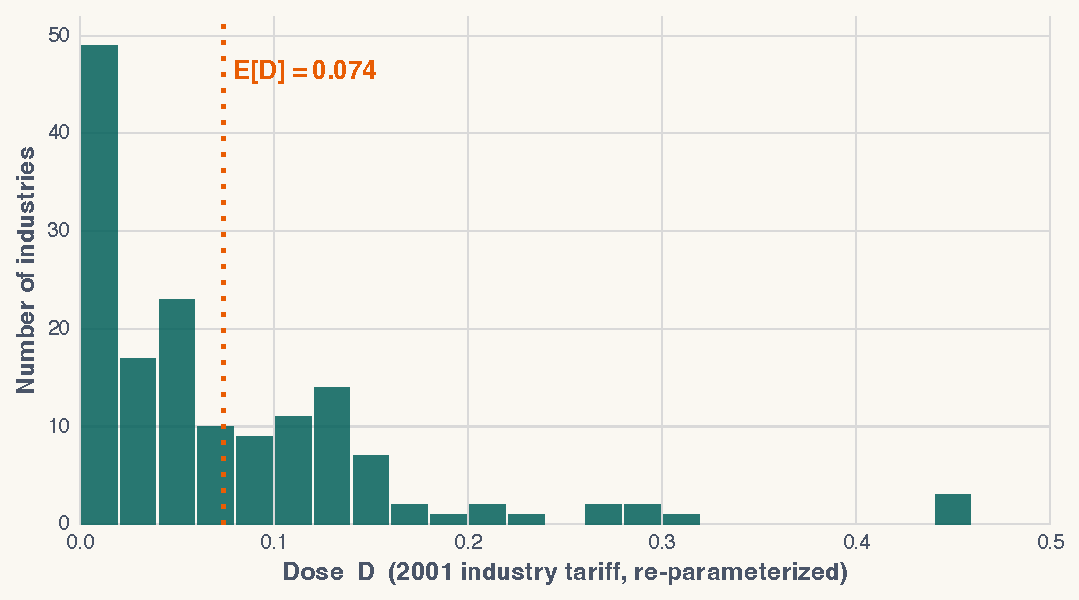
\includegraphics[width=0.78\textwidth,height=0.70\textheight,keepaspectratio]{figures/dxt/01_dose_histogram.pdf}
\end{center}
\vspace{-0.1cm}
\begin{center}
\footnotesize\color{warmgray}\itshape
Tariff cut across 155 Chinese industries. \;\textbf{Mean} $\approx 7\%$; \;range $0$ to $\sim 50\%$.
\end{center}
\end{frame}

\begin{frame}{One coefficient $\widehat\beta^{\text{twfe}}$ carries the entire dose response}
\vspace{0.2cm}

The Lu \& Yu specification is the canonical continuous DiD:
\[
Y_{it} \;=\; \alpha_i \;+\; \gamma_t \;+\; \beta^{\text{twfe}}\,(D_i \cdot \text{Post}_t) \;+\; \varepsilon_{it}
\]

\vspace{0.4cm}

\textbf{One coefficient.} \;No dose-by-dose breakdown. \;No interaction with $D_i^2$ or with bins. \;Just $\beta^{\text{twfe}}$, the slope of $Y$ on $D$ in differenced units.

\vspace{0.4cm}

\textbf{One coefficient, three questions:}
\begin{enumerate}\small\setlength\itemsep{0pt}
  \item Effect of any tariff cut at all?
  \item Effect per percentage point of cut?
  \item Effect at a particular dose, say 10\%?
\end{enumerate}

\vspace{0.3em}
\highlight{$\widehat\beta^{\text{twfe}}$ is supposed to answer all three at once. \;It cannot.}
\end{frame}

\begin{frame}{$\widehat\beta^{\text{twfe}}$ is a weighted average of dose-level effects}
\vspace{0.2cm}

CBS show that the OLS coefficient can be written as:
\[
\widehat\beta^{\text{twfe}} \;=\; \int_0^{\bar d} w(l)\,\cdot\,\big(\text{effect at dose } l\big)\,\,dl
\]

\vspace{0.4cm}

\textbf{This is pure algebra.} \;No potential outcomes yet, no assumptions about identification --- just what the regression \textit{is}, mechanically, as a weighted sum.

\vspace{0.4cm}

\textbf{Four different weights} $w(l)$ can be motivated. \;Each is a real, derivable answer to ``what is $\widehat\beta^{\text{twfe}}$?''

\vspace{0.3em}
\meta{Next: write down the four weight formulas. \;Potential outcomes show up in Part 2.}
\end{frame}

\begin{frame}{The four weight formulas, all at once}
\vspace{0.15cm}
\small
\begin{center}
\begin{tabular}{rl}
\textbf{Level weight:} &
$w^{\text{lev}}(l) \;=\; \dfrac{(l - E[D]) \cdot f_D(l)}{\text{Var}(D)}$ \\[0.7em]
\textbf{Scaled level:} &
$w^{s}(l) \;=\; l \cdot \dfrac{(l - E[D]) \cdot f_D(l)}{\text{Var}(D)}$ \\[0.7em]
\textbf{ACRT weight:} &
$w^{\text{acrt}}(l) \;=\; \dfrac{(E[D \mid D \geq l] - E[D]) \cdot P(D \geq l)}{\text{Var}(D)}$ \\[0.7em]
\textbf{2$\times$2 weight:} &
$w^{2\times 2}(l, h) \;=\; \dfrac{(h - l)^2 \cdot f_D(l) \cdot f_D(h)}{\text{Var}(D)}$ \\
\end{tabular}
\end{center}

\vspace{0.3cm}
\normalsize
\highlight{Same six features of the dose distribution; four ways to recombine them.}
\end{frame}

\begin{frame}{Six ingredients combine into the four weight formulas}
\vspace{0.2cm}

Every weight formula is built from the same six features of the dose distribution:

\vspace{0.4cm}
\begin{enumerate}\small\setlength\itemsep{1pt}
  \item $E[D]$ \;--- the mean dose
  \item $\text{Var}(D)$ \;--- the variance
  \item $f_D(l)$ \;--- the density at dose $l$
  \item $P(D \geq l)$ \;--- the survival probability
  \item $E[D \mid D \geq l]$ \;--- the conditional mean above $l$
  \item $d_L$ \;--- the minimum positive dose
\end{enumerate}

\vspace{0.4cm}
\meta{Same six numbers; four different recombinations.}
\end{frame}

\begin{frame}{Ingredient 1: $E[D]$ anchors every formula}
\vspace{0.1cm}
\begin{center}
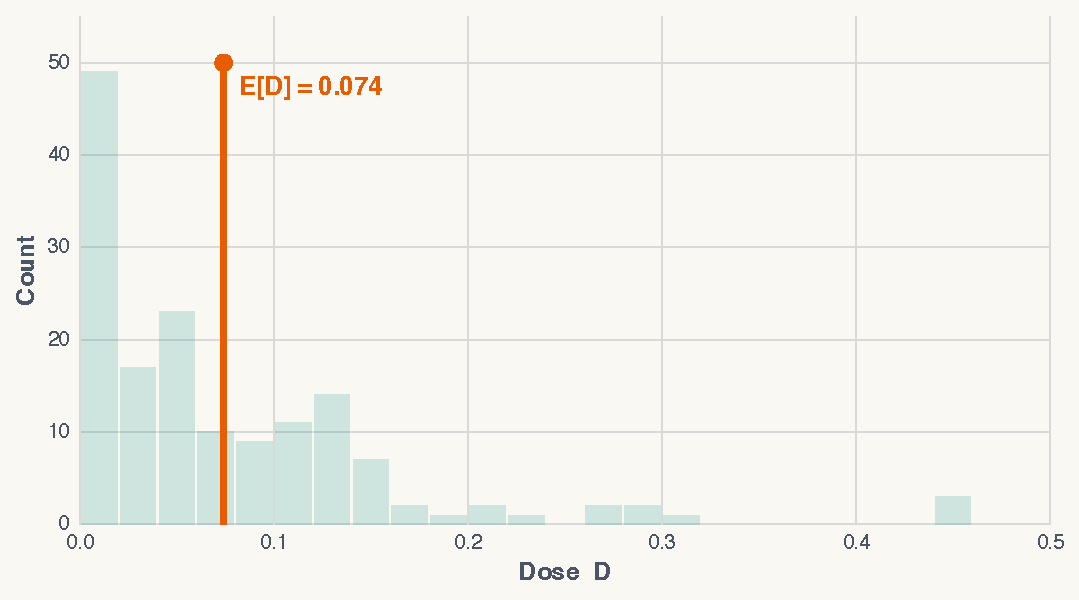
\includegraphics[width=0.78\textwidth,height=0.70\textheight,keepaspectratio]{figures/dxt/02_mean.pdf}
\end{center}
\vspace{-0.05cm}
\begin{center}
\footnotesize\color{warmgray}\itshape
WTO mean dose $\approx 7.1$\%. \;The weights flip sign around this value.
\end{center}
\end{frame}

\begin{frame}{Ingredient 2: $\text{Var}(D)$ sets the scale}
\vspace{0.1cm}
\begin{center}
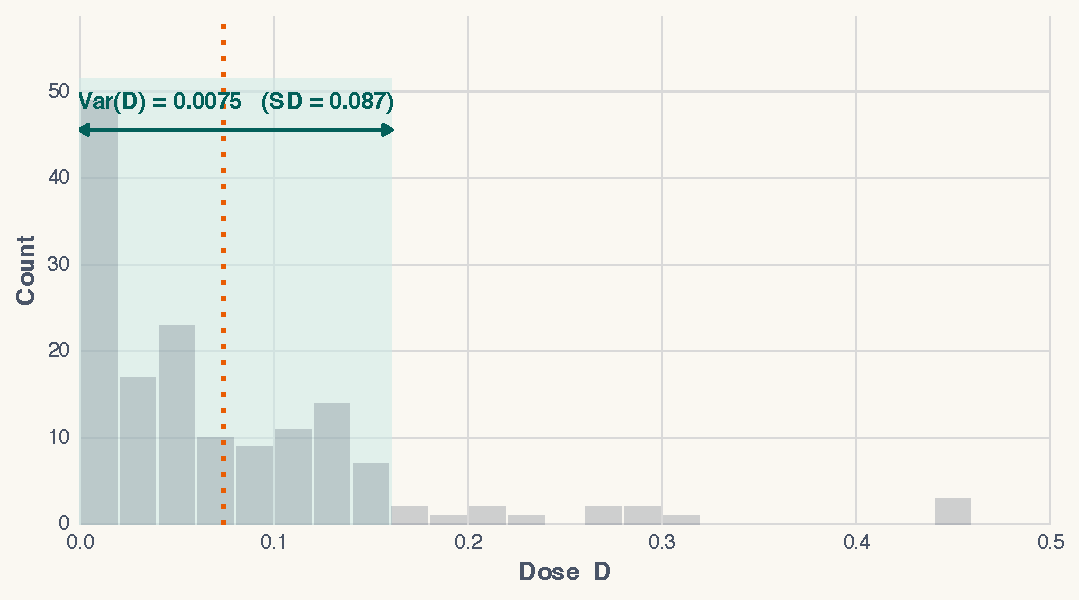
\includegraphics[width=0.78\textwidth,height=0.70\textheight,keepaspectratio]{figures/dxt/03_variance.pdf}
\end{center}
\vspace{-0.05cm}
\begin{center}
\footnotesize\color{warmgray}\itshape
The variance shows up in the denominator of the level weight: \;a higher Var(D) makes the formula scale things down.
\end{center}
\end{frame}

\begin{frame}{Ingredient 3: $f_D(l)$ --- ``where are the industries?''}
\vspace{0.1cm}
\begin{center}
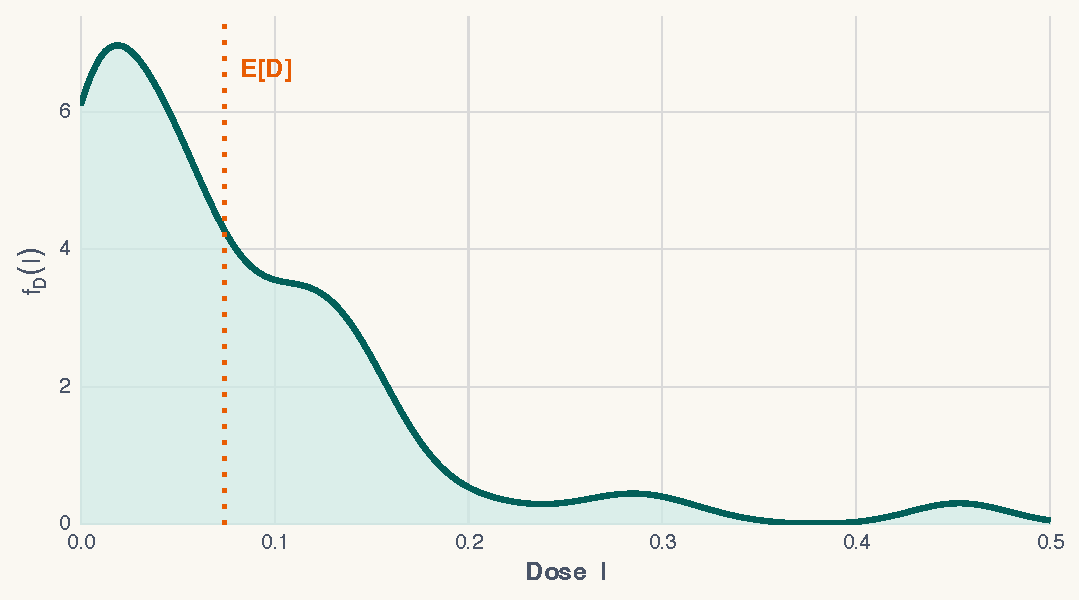
\includegraphics[width=0.78\textwidth,height=0.70\textheight,keepaspectratio]{figures/dxt/04_density.pdf}
\end{center}
\vspace{-0.05cm}
\begin{center}
\footnotesize\color{warmgray}\itshape
The density says where doses cluster. \;The ACRT weight uses $f_D$ directly; the level weight does not.
\end{center}
\end{frame}

\begin{frame}{Ingredient 4: $P(D \geq l)$ --- ``how many above the cutoff?''}
\vspace{0.1cm}
\begin{center}
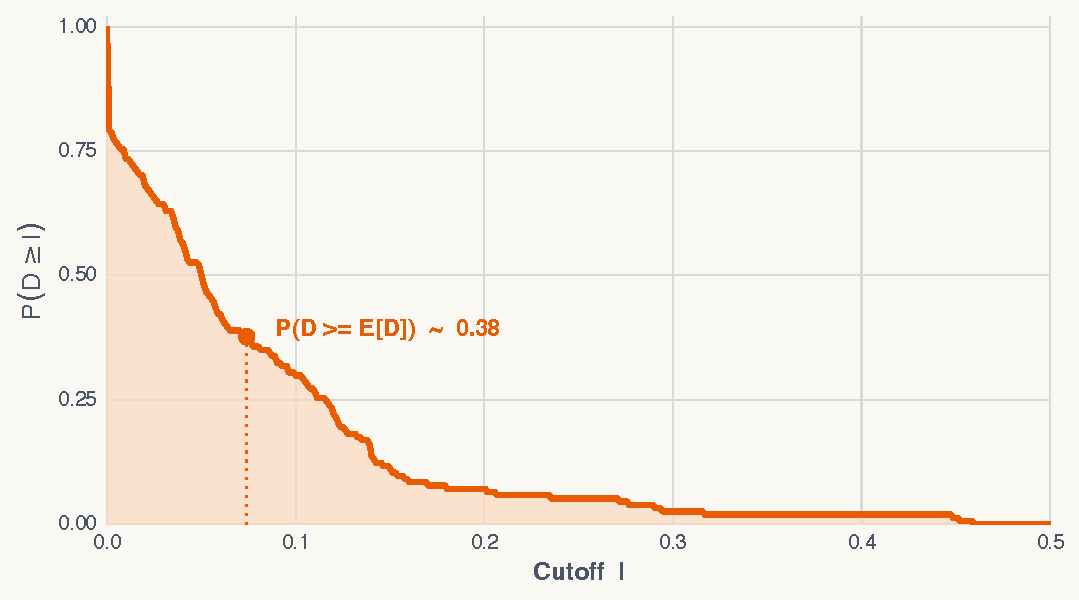
\includegraphics[width=0.78\textwidth,height=0.70\textheight,keepaspectratio]{figures/dxt/05_survival.pdf}
\end{center}
\vspace{-0.05cm}
\begin{center}
\footnotesize\color{warmgray}\itshape
The survival probability counts industries with dose $\geq l$. \;It enters the ACRT formula.
\end{center}
\end{frame}

\begin{frame}{Ingredient 5: $E[D \mid D \geq l]$ tracks the upper tail}
\vspace{0.1cm}
\begin{center}
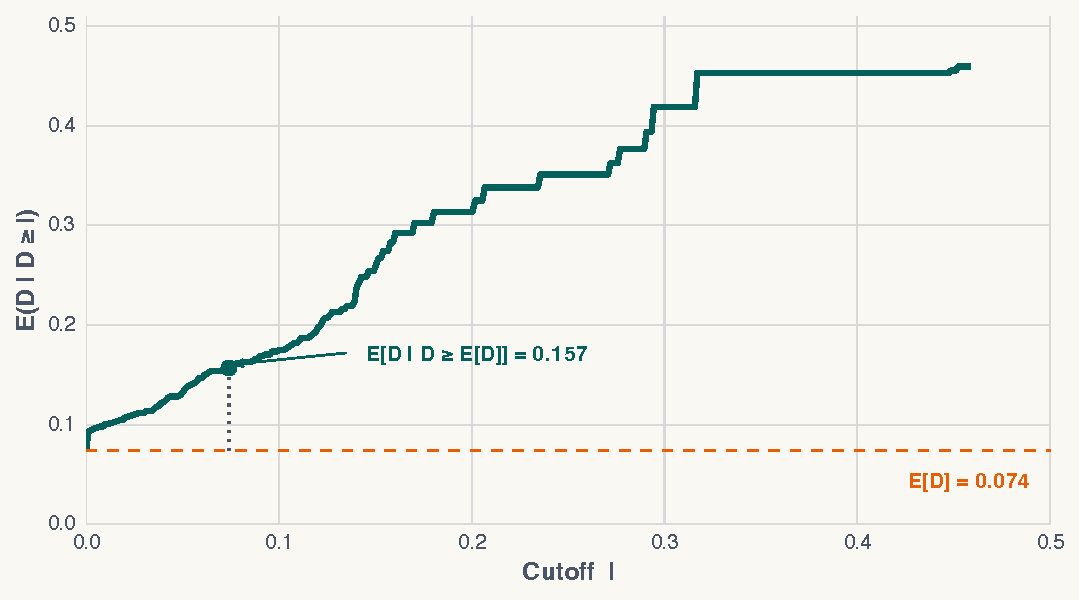
\includegraphics[width=0.78\textwidth,height=0.68\textheight,keepaspectratio]{figures/dxt/06_conditional_mean.pdf}
\end{center}
\vspace{-0.05cm}
\begin{center}
\footnotesize\color{warmgray}\itshape
The conditional mean of dose above cutoff $l$. \;Shows up in the ACRT weight.
\end{center}
\end{frame}

\begin{frame}{Ingredient 6: $d_L$, the minimum positive dose}
\vspace{0.2cm}

The smallest non-zero dose in the data. \;In WTO it is about $0.05$\% (one industry whose 2001 tariff sat just above the 10\% bound). \;Doses $l < d_L$ have weight zero --- no industry experiences that small a cut.

\vspace{0.5cm}

\textbf{Why we name it.} \;Several formulas integrate ``from $d_L$ to $\bar d$.'' \;If you fail to use $d_L$ you can put mass on doses no one ever received --- a textbook source of misinterpretation.

\vspace{0.4em}
\meta{All six ingredients are computed from the cross-section of doses alone --- before the outcome is even loaded.}
\end{frame}

%% ---------- Framing: the regression never changes ----------
\begin{frame}{The regression never changes. \;The question does.}
\vspace{0.4em}

One TWFE regression. \;One $\widehat\beta^{\text{twfe}}$.

\vspace{0.9em}

FWL lets you rewrite that single number as a weighted average --- \textit{four different ways}.

\vspace{0.9em}

\begin{itemize}\setlength\itemsep{0.4em}
  \item Same $\widehat\beta$ each time.
  \item Different \textit{weights} doing the averaging.
  \item Different things being \textit{averaged over}.
\end{itemize}

\vspace{0.7em}

\begin{center}
\highlight{Four rewrites. \;Four implicit questions. \;OLS doesn't tell you which one you asked.}
\end{center}
\end{frame}

%% ---------- Question -> decomposition mapping ----------
\begin{frame}{Four questions, four decompositions}
\vspace{0.2em}
\footnotesize
\begin{center}
\renewcommand{\arraystretch}{1.55}
\begin{tabular}{p{0.34\textwidth} p{0.22\textwidth} p{0.28\textwidth}}
\toprule
\textbf{The question} & \textbf{Target parameter} & \textbf{Decomposition} \\
\midrule
\textbf{Q1.} \;\textit{Effect of the program.} \;Industry at dose $d$ vs.\ untreated. & $\text{ATT}(d \mid d)$ & level weight $w^{\text{lev}}$ \\
\textbf{Q2.} \;\textit{Effect per unit of dose.} & $\dfrac{\text{ATT}(d \mid d)}{d}$ & scaled-level $w^{s}$ \\
\textbf{Q3.} \;\textit{Marginal effect.} \;Tiny nudge at dose $d$. & $\text{ACRT}(d)$ & ACRT weight $w^{\text{acrt}}$ \\
\textbf{Q4.} \;\textit{Two treated industries.} \;Dose $l$ vs.\ dose $h$. & $\text{ATT}(h \mid h, l)$ & 2$\times$2 weight $w^{2\times 2}$ \\
\bottomrule
\end{tabular}
\end{center}

\vspace{0.5em}

\begin{center}
\highlight{All four rewrites equal the same $\widehat\beta$. \;The number doesn't tell you which one you wanted.}
\end{center}
\end{frame}

\begin{frame}{Weight \#1: the level weight $w^{\text{lev}}(l)$}
\vspace{0.05cm}
\[
w^{\text{lev}}(l) \;=\; \frac{(l - E[D]) \cdot f_D(l)}{\text{Var}(D)}
\]
\vspace{-0.25cm}
\begin{center}
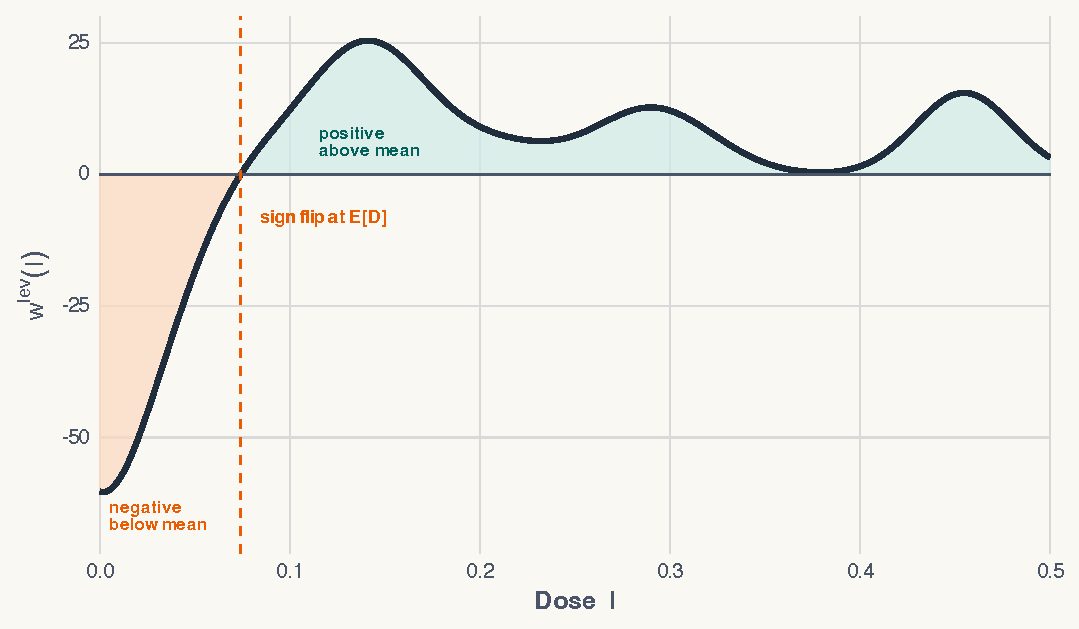
\includegraphics[width=0.72\textwidth,height=0.48\textheight,keepaspectratio]{figures/dxt/07_weight_level.pdf}
\end{center}
\vspace{-0.1cm}
\begin{center}
\footnotesize\color{warmgray}\itshape
Below-mean doses get negative weight; above-mean doses get positive.
\end{center}
\end{frame}

\begin{frame}{Weight \#2: the scaled-level weight $w^{s}(l)$}
\vspace{0.05cm}
\[
w^{s}(l) \;=\; l \cdot \frac{(l - E[D]) \cdot f_D(l)}{\text{Var}(D)}
\]
\vspace{-0.25cm}
\begin{center}
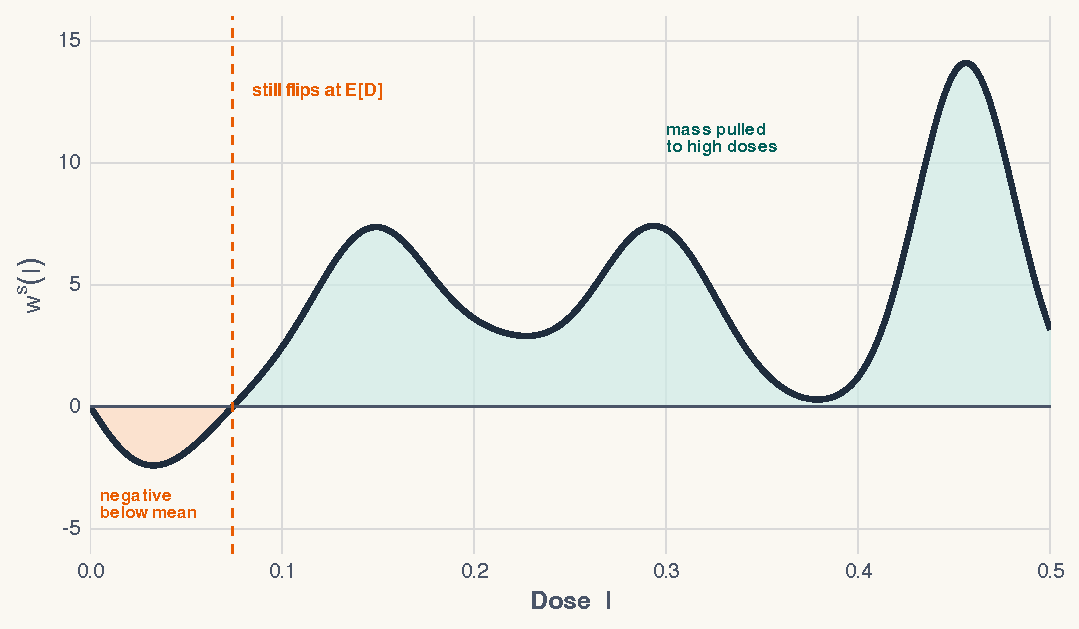
\includegraphics[width=0.72\textwidth,height=0.48\textheight,keepaspectratio]{figures/dxt/08_weight_scaled_level.pdf}
\end{center}
\vspace{-0.1cm}
\begin{center}
\footnotesize\color{warmgray}\itshape
Mass pulled to high doses; sign flip remains. \;Integrates to 1.
\end{center}
\end{frame}

\begin{frame}{Weight \#3: the ACRT weight $w^{\text{acrt}}(l)$}
\vspace{0.05cm}
\[
w^{\text{acrt}}(l) \;=\; \frac{(E[D \mid D \geq l] - E[D]) \cdot P(D \geq l)}{\text{Var}(D)}
\]
\vspace{-0.25cm}
\begin{center}
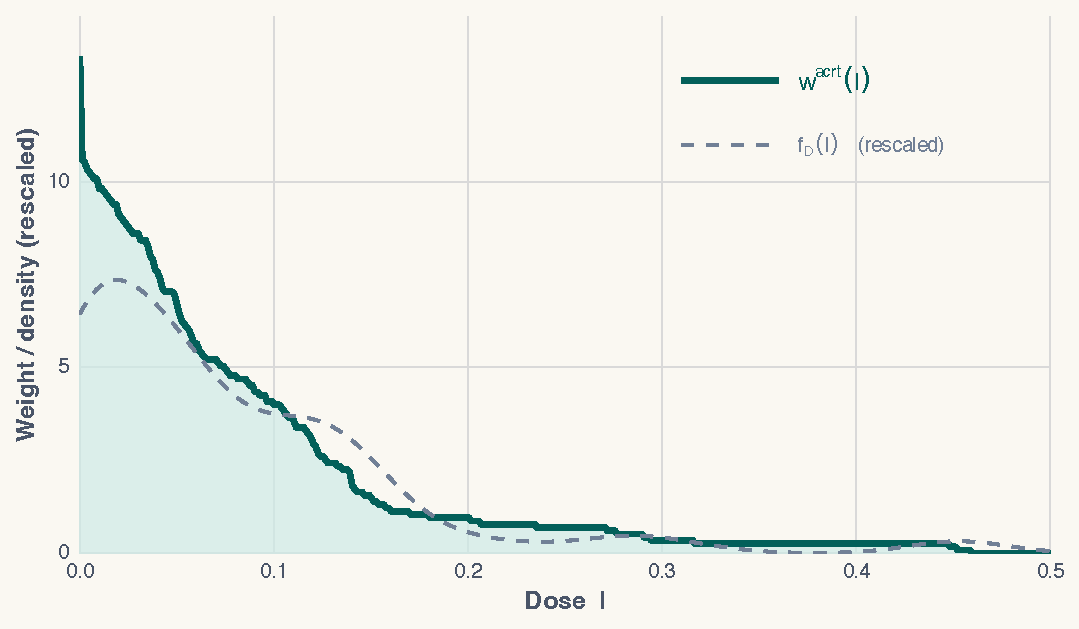
\includegraphics[width=0.72\textwidth,height=0.48\textheight,keepaspectratio]{figures/dxt/09_weight_acrt.pdf}
\end{center}
\vspace{-0.1cm}
\begin{center}
\footnotesize\color{warmgray}\itshape
Non-negative, integrates to 1. \;Shape differs from the density $f_D$.
\end{center}
\end{frame}

\begin{frame}{Weight \#4: the 2$\times$2 weight $w^{2\times 2}(l, h)$}
\vspace{0.05cm}
\[
w^{2\times 2}(l, h) \;=\; \frac{(h - l)^2 \cdot f_D(l) \cdot f_D(h)}{\text{Var}(D)}
\]
\vspace{-0.25cm}
\begin{center}
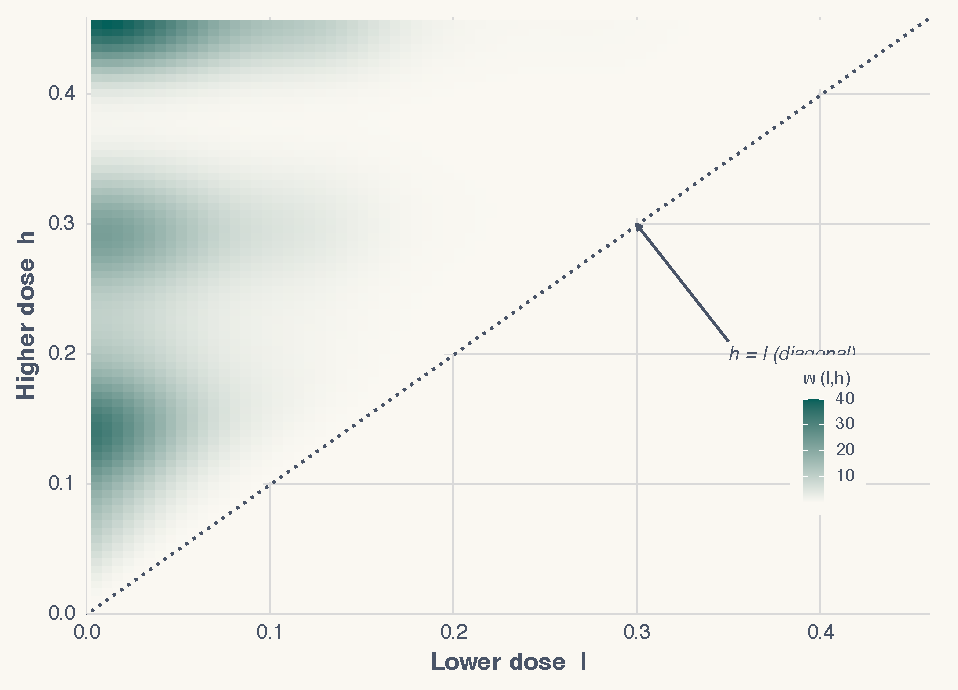
\includegraphics[width=0.62\textwidth,height=0.48\textheight,keepaspectratio]{figures/dxt/10_weight_2x2_heatmap.pdf}
\end{center}
\vspace{-0.1cm}
\begin{center}
\footnotesize\color{warmgray}\itshape
Far-apart pairs get the most weight; $(h - l)^2$ shows up visually.
\end{center}
\end{frame}

\begin{frame}{Same dose distribution, four different stories}
\vspace{0.1cm}
\begin{center}
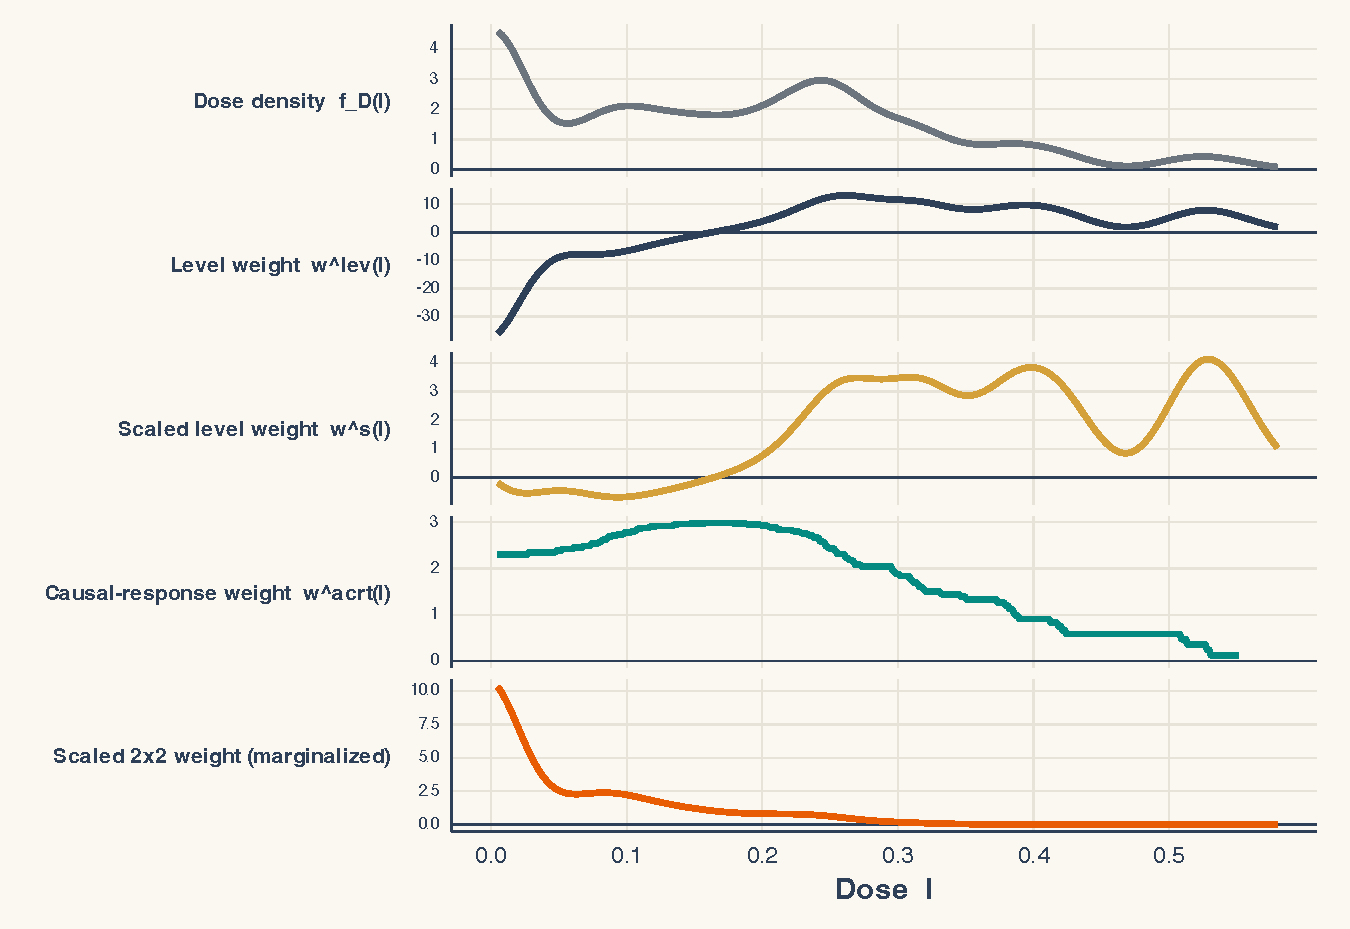
\includegraphics[width=0.78\textwidth,height=0.70\textheight,keepaspectratio]{figures/dxt/11_synthesis.pdf}
\end{center}
\vspace{-0.05cm}
\begin{center}
\footnotesize\color{warmgray}\itshape
Four overlaid weights, same distribution. \;$\widehat\beta^{\text{twfe}}$ is all of them at once.
\end{center}
\end{frame}

%% =========================================================================
%%   FWL reconstruction on Kyle's WTO sample
%% =========================================================================

\begin{frame}[fragile]{Let's verify it with data}
\vspace{0.4em}

We've described the weights. \;Now let's actually compute them and rebuild $\widehat\beta^{\text{twfe}}$ by hand.

\vspace{0.8em}

Three steps:
\begin{enumerate}\setlength\itemsep{0.3em}
  \item Run OLS of $\Delta\ln\text{Theil}$ on dose. \;Save $\widehat\beta_{\text{OLS}}$.
  \item Compute per-industry level weights $W_i = \dfrac{D_i - \bar D}{\sum_j (D_j - \bar D)^2}$.
  \item Form $\sum_i W_i \cdot \Delta\ln\text{Theil}_i$ and compare.
\end{enumerate}

\vspace{0.5em}
\begin{center}
\highlight{If FWL is right, the two numbers are identical.}
\end{center}

\vspace{0.5em}
\begin{lstlisting}[basicstyle=\ttfamily\tiny\color{warmgray},frame=none,backgroundcolor=\color{white}]
Labs/China-WTO/twfe_reconstruction.R    # R version
Labs/China-WTO/twfe_reconstruction.do   # Stata version
\end{lstlisting}
\end{frame}

\begin{frame}[fragile]{The reconstruction in Stata}
\footnotesize
\begin{lstlisting}[language={[ANSI]C},basicstyle=\ttfamily\scriptsize]
* (1) beta_hat from OLS
reg Delta_ln_theil dose
local beta_ols = _b[dose]

* (2) Per-industry level weights  W_i = (D_i - Dbar) / SS_D
egen D_bar = mean(dose)
gen  W_num = dose - D_bar
egen SS_D  = total(W_num^2)
gen  W     = W_num / SS_D

* (3) Reconstruct beta_hat by hand
gen  contrib = W * Delta_ln_theil
egen beta_manual = total(contrib)
\end{lstlisting}

\vspace{0.4em}
\begin{center}
\highlight{R companion at \texttt{Labs/China-WTO/twfe\_reconstruction.\{R,do\}}}
\end{center}
\end{frame}

\begin{frame}{$\widehat\beta^{\text{twfe}}$ is the weighted average. \;Exactly.}
\vspace{0.4em}
\begin{center}
\renewcommand{\arraystretch}{1.5}
\begin{tabular}{l@{\hspace{1.5em}}r}
\toprule
\textbf{Quantity} & \textbf{Value} \\
\midrule
$\widehat\beta_{\text{OLS}}$ from \texttt{reg Delta\_ln\_theil dose} & $-0.493524$ \\
$\sum_i W_i \cdot \Delta\ln\text{Theil}_i$ \;(weighted sum) & $-0.493524$ \\
\midrule
$|\widehat\beta_{\text{OLS}} - \sum_i W_i \cdot \Delta\ln\text{Theil}_i|$ & $5.55 \times 10^{-17}$ \\
\bottomrule
\end{tabular}
\end{center}

\vspace{0.6em}
\begin{center}
\highlight{Numerically identical to machine precision.}
\end{center}

\vspace{0.2em}
\begin{center}
The decomposition \textit{is} the regression.
\end{center}
\end{frame}

\begin{frame}{Negative weights aren't a bug --- they're the price}
\vspace{0.4em}

\begin{itemize}\setlength\itemsep{0.5em}
  \item \textbf{Q1, Q2 (level, scaled-level).} \;Clean comparison: treated dose $d$ vs.\ untreated. \;Weights forced to sum to zero $\Rightarrow$ below-mean doses get \textit{negative} weights.
  \item \textbf{Q4 (2$\times$2).} \;Weights non-negative, integrate to 1 --- but compare two \textit{treated} industries to each other. \;A forbidden contrast.
  \item \textbf{Q3 (ACRT).} \;In between: non-negative weights, but the answer is a derivative, not a level.
\end{itemize}

\vspace{0.5em}
\begin{center}
\highlight{Clean comparisons cost you negative weights. \;Tidy weights cost you forbidden comparisons. \;Pick your poison.}
\end{center}
\end{frame}

\begin{frame}{The takeaway from the decomposition}
\vspace{0.2cm}

\textbf{$\widehat\beta^{\text{twfe}}$ is well-defined.} \;It is a sample statistic. \;But:

\vspace{0.4cm}

\begin{itemize}\small\setlength\itemsep{2pt}
  \item It is \textit{not} the average dose effect \;(that would be $\int f_D(l)\,\text{ATT}(l \mid l)\,dl$).
  \item It is \textit{not} the ACRT \;(that uses $w^{\text{acrt}}$, not $w^{\text{lev}}$).
  \item It \textit{is} a weighted combination, with sign-flipping weights, of dose-specific effects.
\end{itemize}

\vspace{0.5cm}

\highlight{The path forward.} \;Pick the target parameter first. \;Estimate that parameter. \;Don't read $\widehat\beta^{\text{twfe}}$ as ``the'' dose effect.

\vspace{0.4em}
\meta{Part 2 defines those target parameters. \;Part 3 estimates them.}
\end{frame}

\begin{frame}{Play with the decomposition: the \texttt{baconplus} Shiny app}
\vspace{0.2cm}

\textbf{Interactive companion} to everything we just did:
\begin{center}
\href{https://scunning1975.github.io/baconplus/}{\color{ocean}\underline{\texttt{https://scunning1975.github.io/baconplus/}}}
\end{center}

\vspace{0.3cm}

\textbf{What it does.} \;Slider-based exploration of the TWFE decomposition on 155 simulated industries with a tariff-cut dose mimicking Lu \& Yu (2015):
\begin{itemize}\small\setlength\itemsep{1pt}
  \item Move the kernel bandwidth and watch $f_D(l)$ re-shape.
  \item See the level weight $w^{\text{lev}}(l)$, the scaled-level $w^s(l)$, and the ACRT weight $w^{\text{acrt}}(l)$ rebuild in real time.
  \item Reassemble $\widehat\beta^{\text{twfe}}$ from any of the four weight formulas.
\end{itemize}

\vspace{0.3em}
\meta{Source: \;\href{https://github.com/scunning1975/baconplus}{github.com/scunning1975/baconplus} --- CBS continuous-DiD TWFE decomposition implementation.}
\end{frame}

% =============================================================================
% PART III — Potential outcomes and building blocks
% =============================================================================

\remixsection{Part 2: \\ Potential outcomes and \\ building blocks}

\begin{frame}{ATT, but for a continuous dose}
\vspace{0.2cm}

\textbf{Recall the binary ATT:}
\[
\text{ATT} \;=\; \mathbb{E}\big[\,Y_{it}(1) - Y_{it}(0) \mid D_i = 1,\,\text{Post}_t\,\big]
\]

\vspace{0.4cm}

\textbf{With a continuous dose} we need a richer object. \;Each unit has a potential outcome \textit{at every possible dose}: $Y_{it}(d)$ for $d \in [0, \bar d]$.

\vspace{0.4cm}

\textbf{Two natural parameters:}
\begin{enumerate}\small\setlength\itemsep{1pt}
  \item Effect of \textit{being at} dose $d$ vs being at zero. \;(``ATT at dose $d$'')
  \item Effect of \textit{moving} from dose $d$ to dose $d + \Delta$. \;(``causal response'')
\end{enumerate}

\vspace{0.3em}
\highlight{These are not the same thing.}
\end{frame}

\begin{frame}{Dosage parameters give us a multitude of ATTs}
\vspace{0.2cm}

\begin{block}{ATT for a given dose}
\[
\text{ATT}(d \mid d) \;=\; \mathbb{E}\big[\,Y_{it}(d) - \textcolor{ocean}{Y_{it}(0)} \mid D_i = d\,\big]
\]
\end{block}

\vspace{0.4cm}

\textbf{Read it as:} \;``The ATT of dose $d$ for the group of units that actually \textit{received} dose $d$, using zero dose as the counterfactual.''

\vspace{0.3cm}

\textbf{Example.} \;What is the effect of being 100 km from a hospital, compared to being 0 km? \;Comparison is no-dose; population is the units actually 100 km away.

\vspace{0.3em}
\meta{One ATT per dose; the full set is the dose-response curve.}
\end{frame}

\begin{frame}{ATT for a given dose: the aspirin example (1)}
\begin{center}
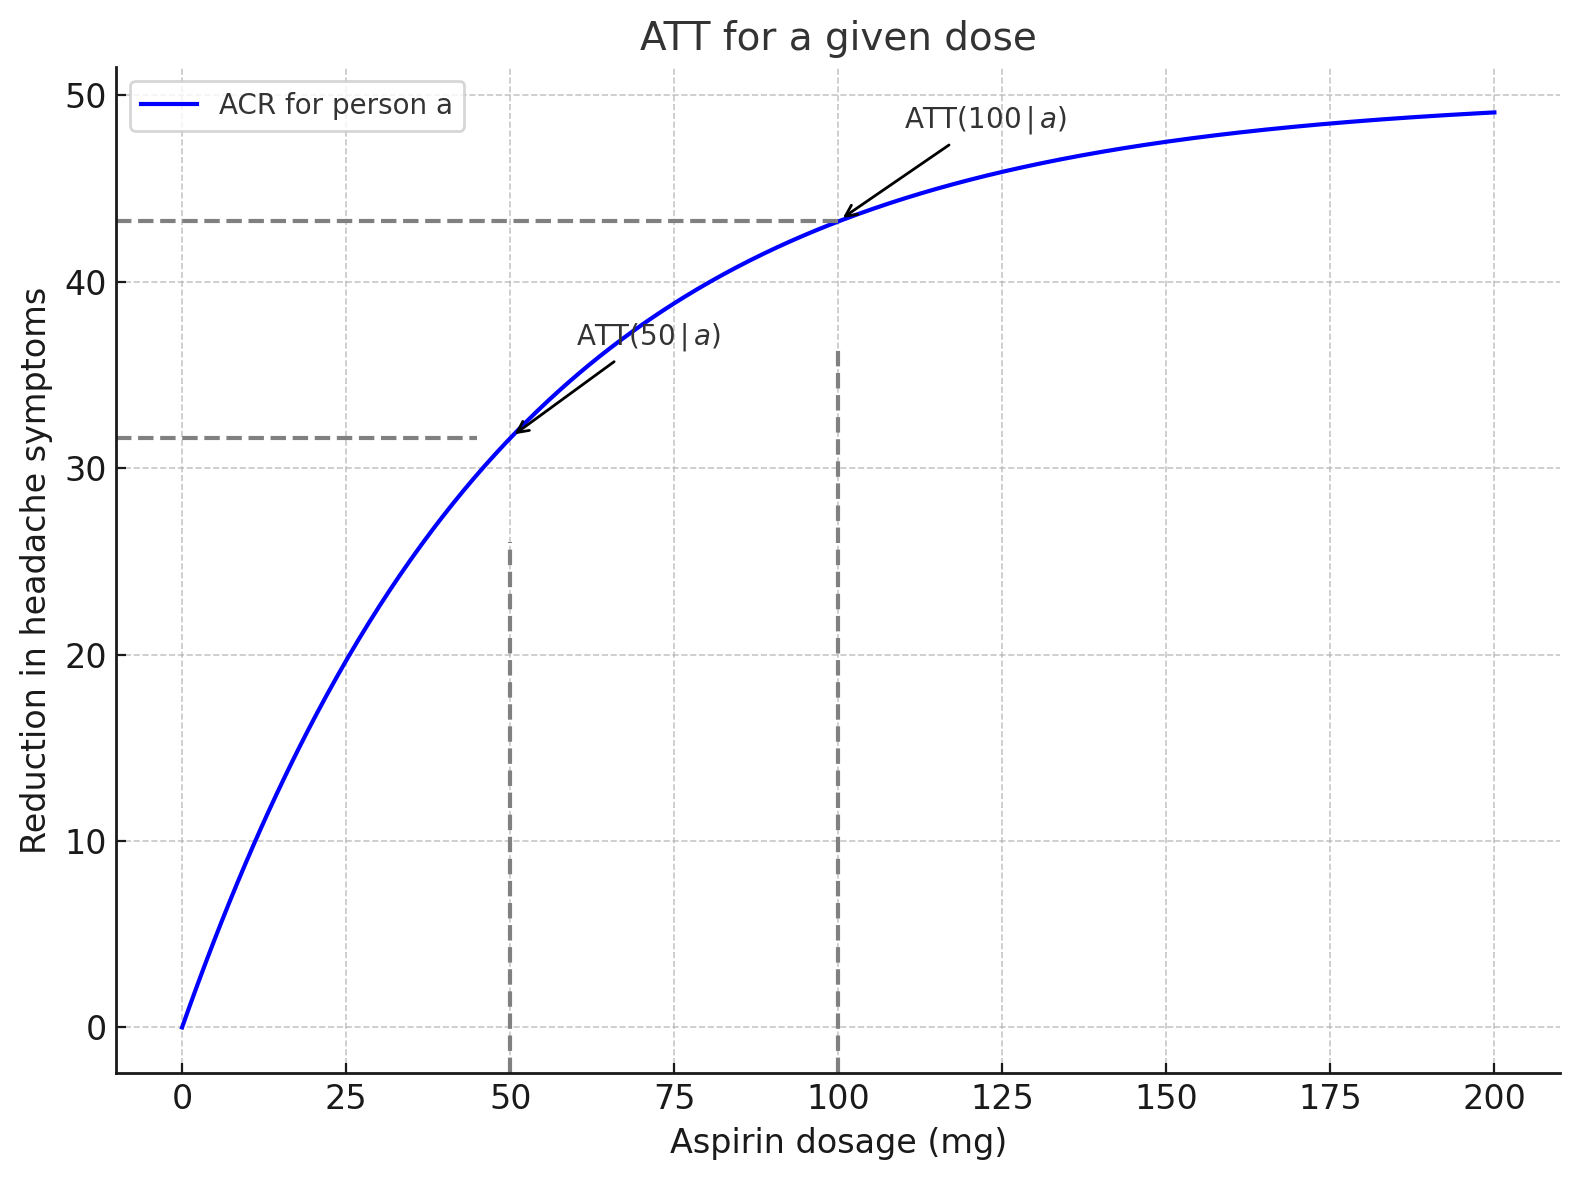
\includegraphics[width=0.6\textwidth,height=0.70\textheight,keepaspectratio]{figures/dxt/acrt_fig1.png}
\end{center}
\vspace{-0.1cm}
\begin{center}
\footnotesize\color{warmgray}\itshape
One person, one outcome (headache pain). \;At 50 mg, the effect is 31; at 100 mg, the effect is 44.
\end{center}
\end{frame}

\begin{frame}{ATT for a given dose: the aspirin example (2)}
\begin{center}
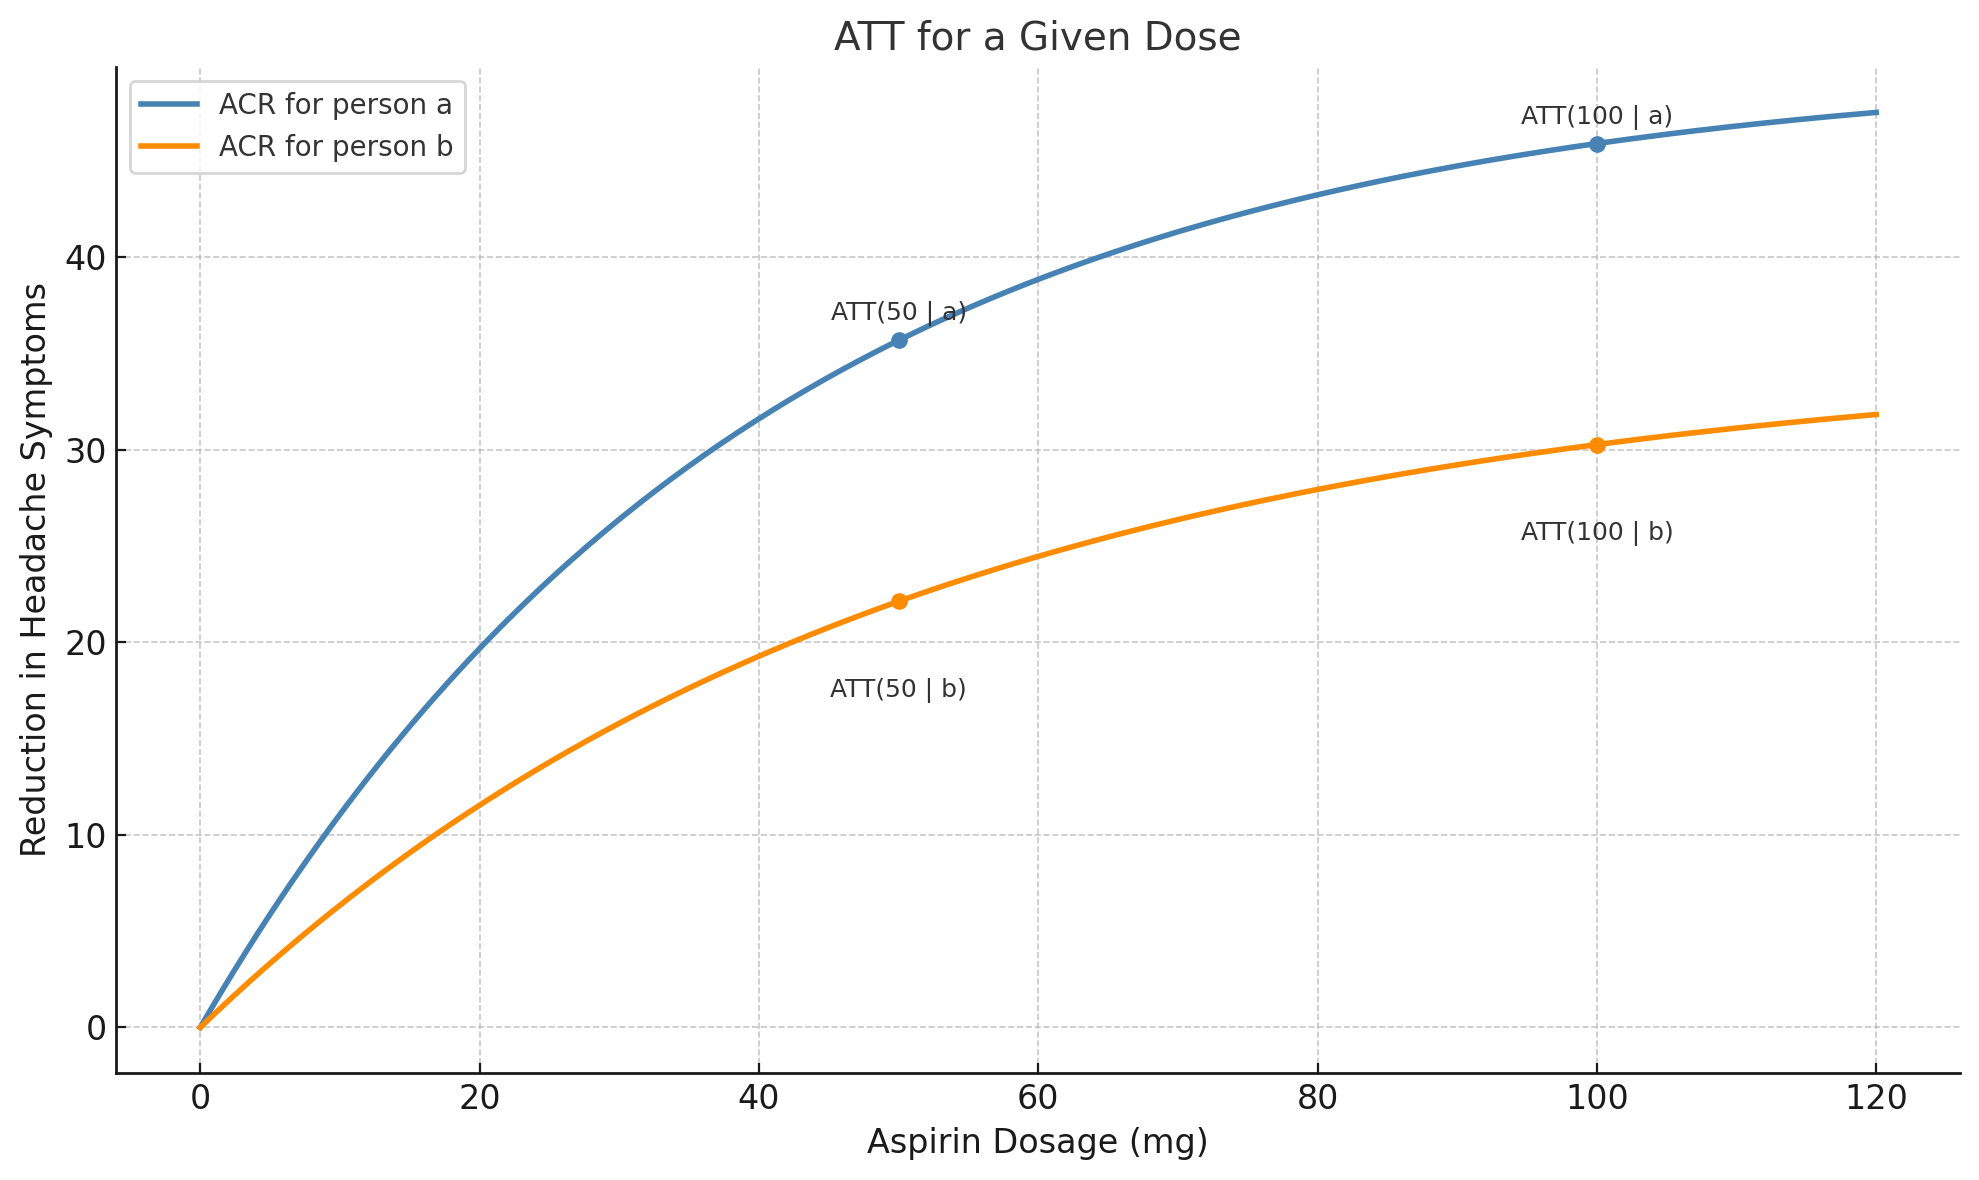
\includegraphics[width=0.6\textwidth,height=0.70\textheight,keepaspectratio]{figures/dxt/acrt_fig2.png}
\end{center}
\vspace{-0.1cm}
\begin{center}
\footnotesize\color{warmgray}\itshape
$\text{ATT}(50 \mid 50)$ vs $\text{ATT}(100 \mid 100)$: \;two separate ATT numbers, each comparing dose $d$ to zero dose.
\end{center}
\end{frame}

\begin{frame}{Moving along the dosage is \emph{not} the ATT}
\vspace{0.2cm}
\begin{center}
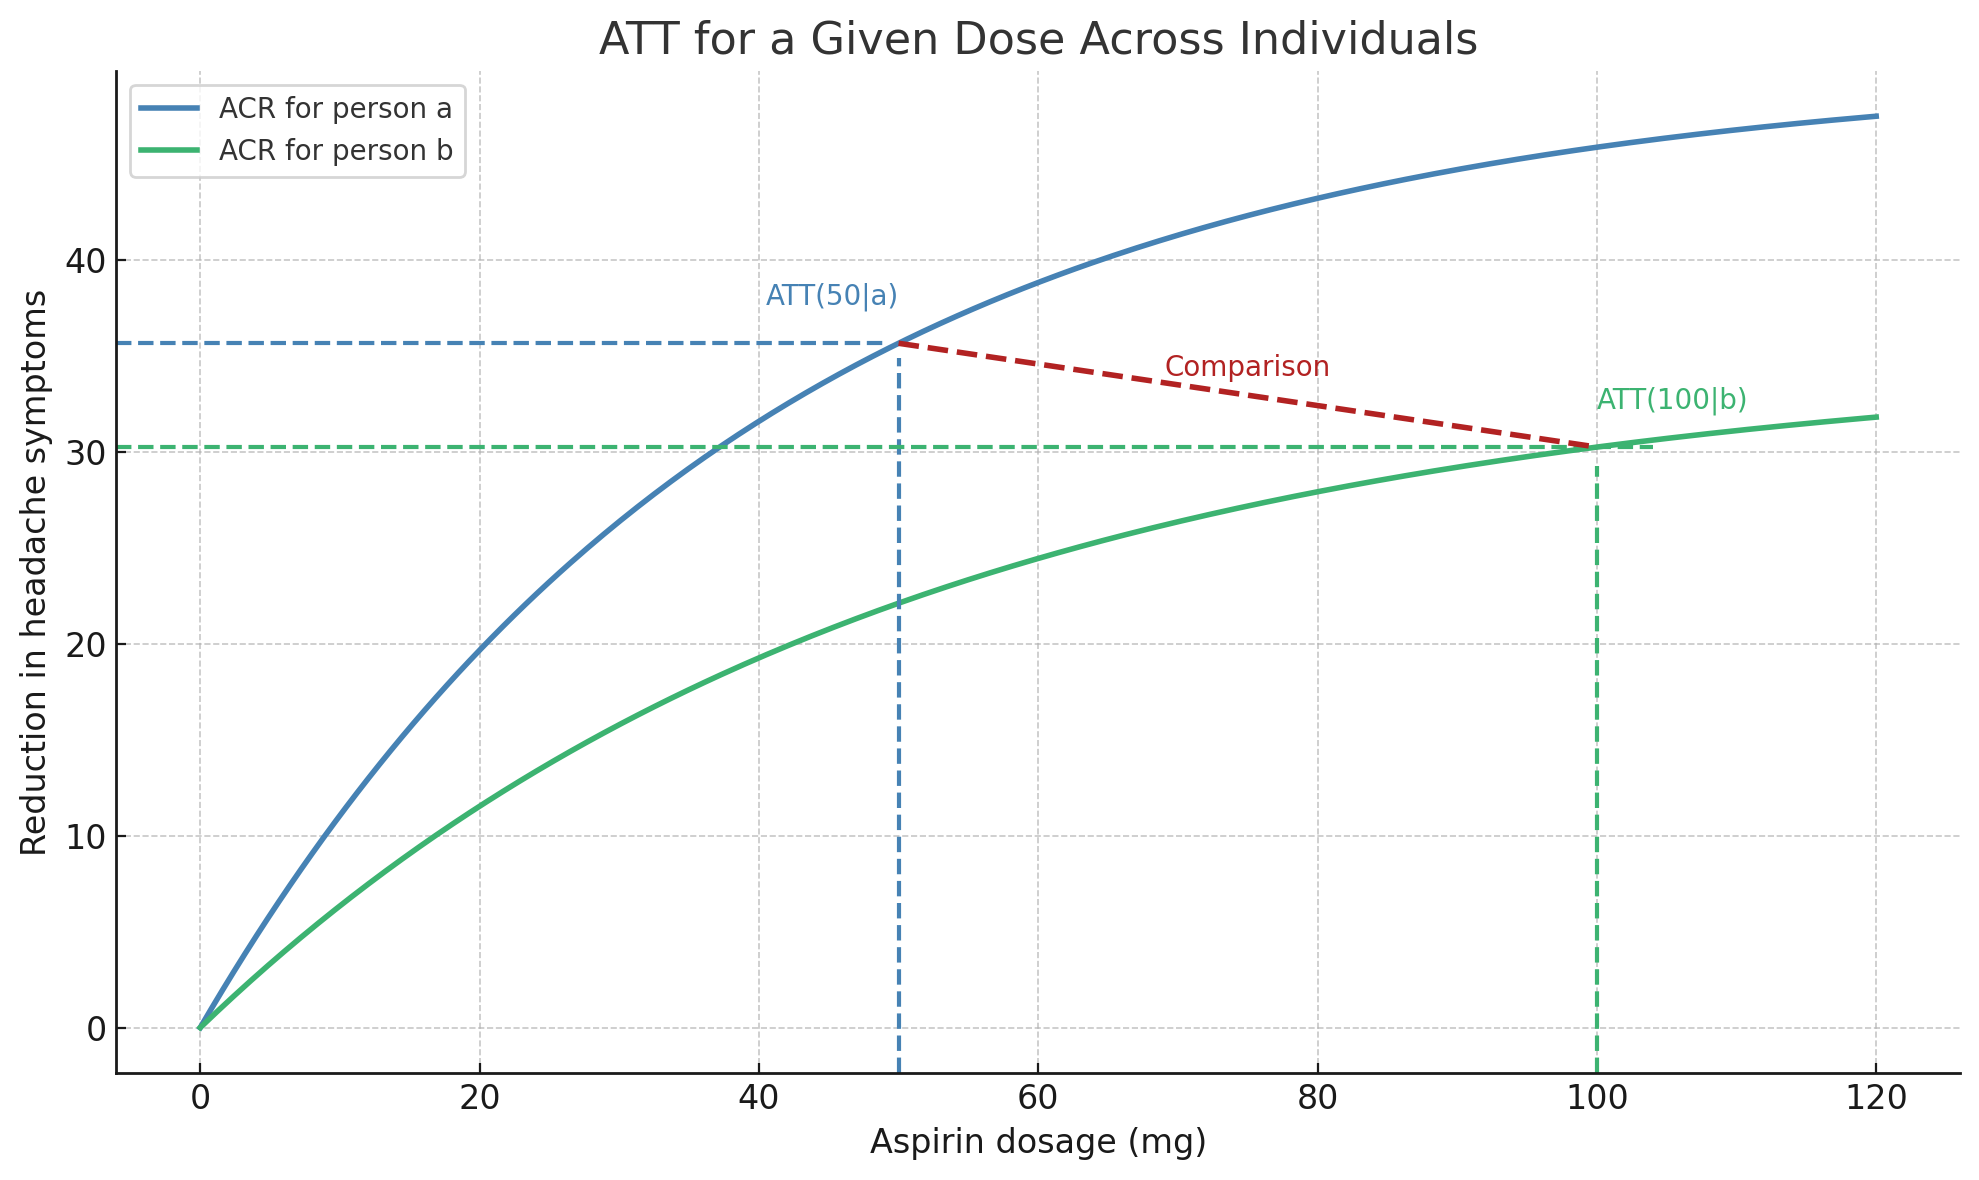
\includegraphics[width=0.6\textwidth,height=0.70\textheight,keepaspectratio]{figures/dxt/acrt_fig2b.png}
\end{center}
\vspace{-0.1cm}
\begin{center}
\footnotesize\color{warmgray}\itshape
The \textit{difference between} $\text{ATT}(100)$ and $\text{ATT}(50)$ is \;a slope, not an ATT. \;It's a marginal effect along the dose response curve.
\end{center}
\end{frame}

\begin{frame}{The Average Causal Response on the Treated --- ACRT}
\vspace{0.2cm}

\begin{block}{ACRT}
\[
\text{ACRT}(d) \;=\; \frac{\partial}{\partial d}\,\mathbb{E}\big[\,Y_{it}(d) \mid D_i = d\,\big]
\]
\end{block}

\vspace{0.4cm}

\textbf{Read it as:} \;``How much does the outcome change if I bump dose up by a tiny amount, evaluated at units actually receiving that dose?''

\vspace{0.4cm}

\textbf{A slope, not a level.} \;A marginal effect: mg per mg, km per km, point per point.

\vspace{0.2em}
\meta{Angrist \& Imbens (1995) defined the IV analog, ACR.}
\end{frame}

\begin{frame}{ACRT as a derivative}
\begin{center}
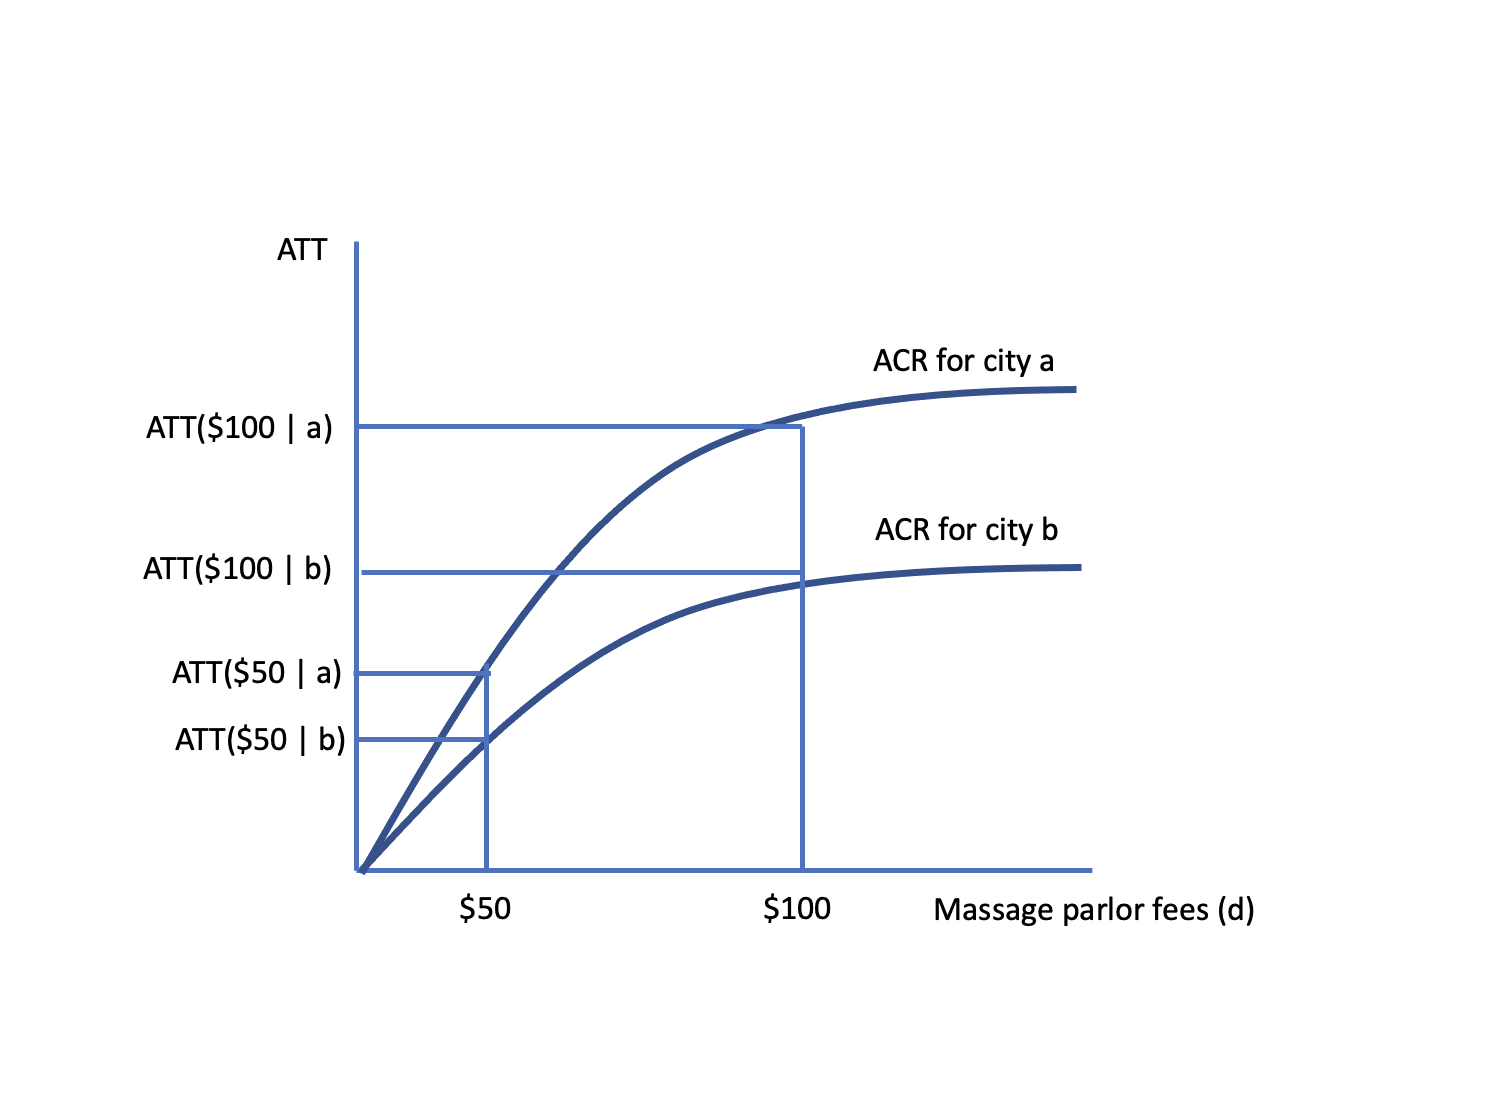
\includegraphics[width=0.6\textwidth,height=0.70\textheight,keepaspectratio]{figures/dxt/acrt_fig2c.png}
\end{center}
\vspace{-0.1cm}
\begin{center}
\footnotesize\color{warmgray}\itshape
ACRT($d$) is the slope of the ATT-dose curve at dose $d$ --- the marginal effect of one more unit of treatment.
\end{center}
\end{frame}

\begin{frame}{Two different parameters, two different questions}
\begin{center}
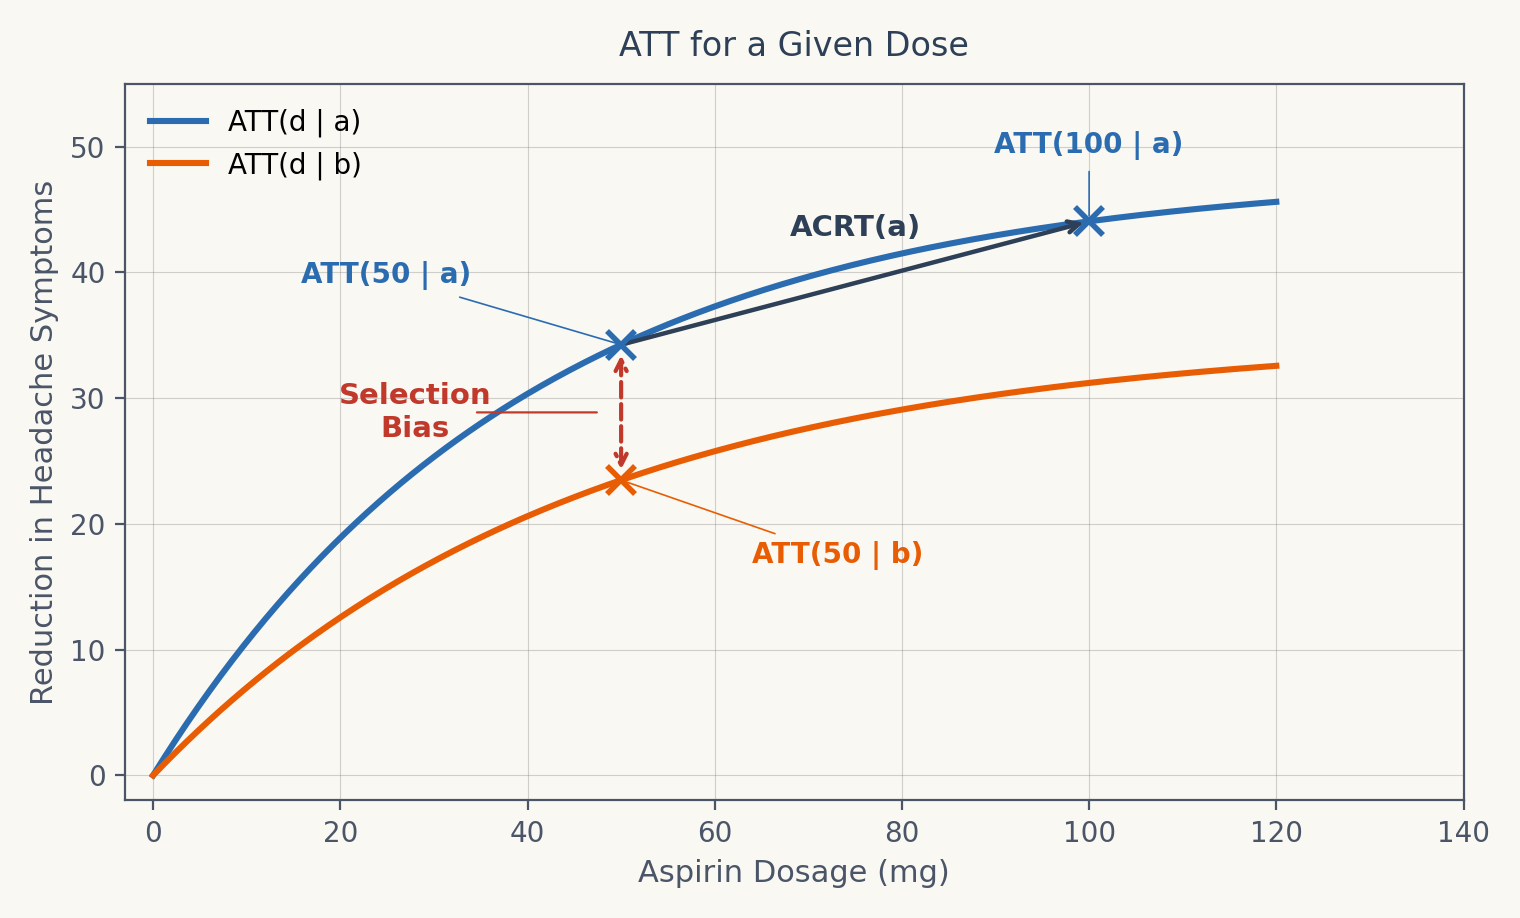
\includegraphics[width=0.6\textwidth,height=0.70\textheight,keepaspectratio]{figures/dxt/acrt_fig2d.png}
\end{center}
\vspace{-0.1cm}
\begin{center}
\footnotesize\color{warmgray}\itshape
$\text{ATT}(d \mid d)$ is a level; ACRT($d$) is a slope. \;Different objects, often confused.
\end{center}
\end{frame}

\begin{frame}{Identification: assumptions for ATT($d \mid d$)}
\vspace{0.2cm}

\textbf{A1. No Anticipation.} \;Treatment doesn't move outcomes before it begins.
\[
Y_{it}(d) \;=\; Y_{it}(0) \quad \text{for all } t < g_i
\]

\vspace{0.3cm}

\textbf{A2. Standard Parallel Trends (PT).} \;The trend in $Y_{it}(0)$ is the same for treated units regardless of their realized dose:
\[
\mathbb{E}\big[\Delta Y_{it}(0) \mid D_i = d\big] \;=\; \mathbb{E}\big[\Delta Y_{it}(0) \mid D_i = 0\big]
\]

\vspace{0.4cm}

\highlight{This gives identification of $\text{ATT}(d \mid d)$ for each $d > 0$.} \;The level-effect dose-response curve, against the no-dose counterfactual.

\vspace{0.4em}
\meta{Standard PT is the natural extension of binary-PT to a continuous setting.}
\end{frame}

%% ---------- The 2x2 falls out of No Anticipation ----------
\begin{frame}{No Anticipation $\Rightarrow$ baseline is $Y(0)$ for everyone}
\vspace{0.5em}

A1 says: \;pre-treatment potential outcomes do not depend on the future dose.

\vspace{0.8em}

Combined with the data structure (no one is observationally treated yet in the pre-period), this gives:
\[
Y_{i,\text{pre}} \;=\; Y_{i,\text{pre}}(0) \quad \text{for every unit } i, \;\text{including those who get } D_i > 0 \text{ later.}
\]

\vspace{0.8em}

\textbf{Why this matters.} \;Every DiD comparison the model can express is mechanically a 2$\times$2:
\begin{itemize}\setlength\itemsep{0.2em}
  \item \textit{before} = the common untreated trajectory (both groups).
  \item \textit{after} = treated units show $Y(d)$; control units stay on $Y(0)$.
\end{itemize}

\vspace{0.4em}
\begin{center}
\highlight{The $(D \times \text{Post})$ interaction in TWFE is the mechanical consequence.}
\end{center}
\end{frame}

\begin{frame}{Identification: ACRT requires more --- ``Strong PT''}
\vspace{0.2cm}

\textbf{A2$'$. Strong Parallel Trends.} \;The \textit{counterfactual} trend at \textit{every} dose is the same across treatment groups:
\[
\mathbb{E}\big[\Delta Y_{it}(d) - \Delta Y_{it}(0) \mid D_i = d'\big] \;=\; \mathbb{E}\big[\Delta Y_{it}(d) - \Delta Y_{it}(0) \mid D_i = d\big]
\]

\vspace{0.4cm}

\textbf{In words.} \;The treatment effect of dose $d$ on a unit that actually received dose $d$ equals the treatment effect of dose $d$ on a unit that received dose $d'$.

\vspace{0.4cm}

\highlight{This rules out selection on gains across doses.} \;Strong PT is a substantial restriction; standard PT alone does not yield the ACRT.

\vspace{0.4em}
\meta{Under standard PT we identify the \textit{level curve}; \;under strong PT we identify the \textit{slope} as the ACRT.}
\end{frame}

\begin{frame}{Why strong PT is stronger: a thought experiment}
\vspace{0.2cm}

Suppose two industries: \;A chose a 10\% tariff cut; \;B chose a 30\% cut. \;Dose was not random.

\vspace{0.3cm}

\textbf{Standard PT} says: \;A and B would have had the same \textit{baseline} trend, absent any cut.

\vspace{0.3cm}

\textbf{Strong PT} says, in addition: \;\textit{if A and B both faced a 20\% cut}, they'd respond identically.

\vspace{0.3cm}

\highlight{Strong PT rules out selection on dose-response gains.}
\end{frame}

\begin{frame}{A discrete multi-valued example: pills, groups, DiD}
\vspace{0.2cm}

To see how DiD operates on dose groups, drop continuous and consider a \textit{multi-valued} discrete dose: $D \in \{0, 1, 2\}$.

\vspace{0.4cm}

\textbf{Setting.} \;Three groups of patients: untreated ($D = 0$), one pill ($D = 1$), two pills ($D = 2$). \;The discrete case bridges binary and continuous --- same ideas, finite groups.

\vspace{0.4cm}

\textbf{Next slides.} \;Dose-by-dose ATTs, first-differences, the DiD, what's actually identified.
\end{frame}

\begin{frame}{Discrete: raw outcomes by dose group}
\begin{center}
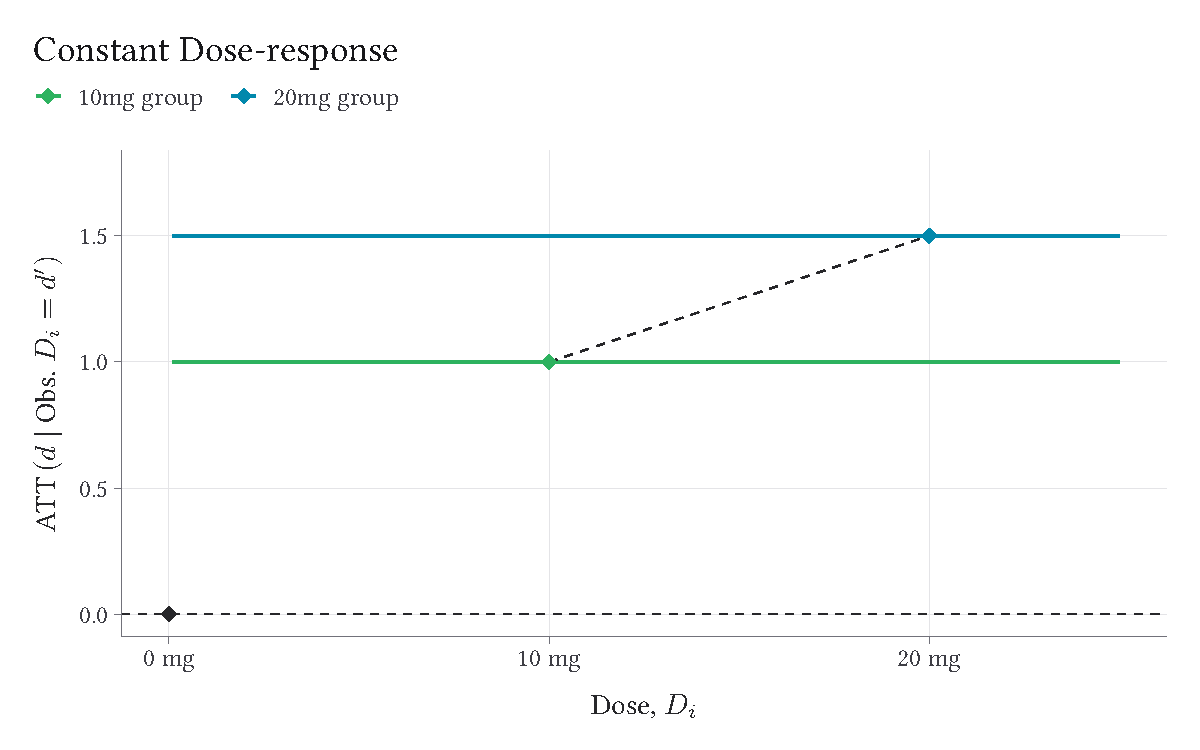
\includegraphics[width=0.78\textwidth,height=0.70\textheight,keepaspectratio]{figures/dxt/discrete_te_constant.pdf}
\end{center}
\begin{center}
\footnotesize\color{warmgray}\itshape
Three dose groups (0, 1, 2 pills). \;Their pre-period levels and trends are all parallel --- this is the no-treatment-effect benchmark.
\end{center}
\end{frame}

\begin{frame}{Discrete: with treatment effects (linear, homogeneous)}
\begin{center}
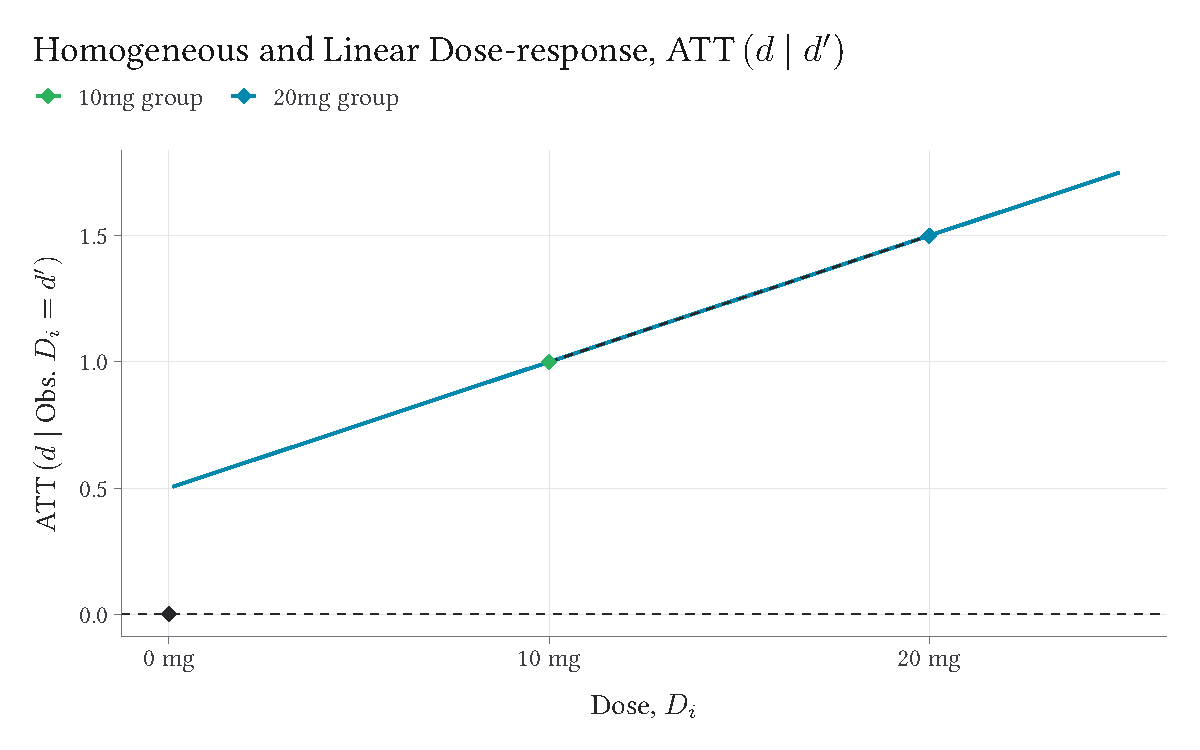
\includegraphics[width=0.78\textwidth,height=0.70\textheight,keepaspectratio]{figures/dxt/discrete_te_linear_homogenous.pdf}
\end{center}
\begin{center}
\footnotesize\color{warmgray}\itshape
Dose-1 group lifts by $\delta$; dose-2 group lifts by $2\delta$. \;Effects linear in dose; everyone responds the same way.
\end{center}
\end{frame}

\begin{frame}{Discrete: with heterogeneity in the dose response}
\begin{center}
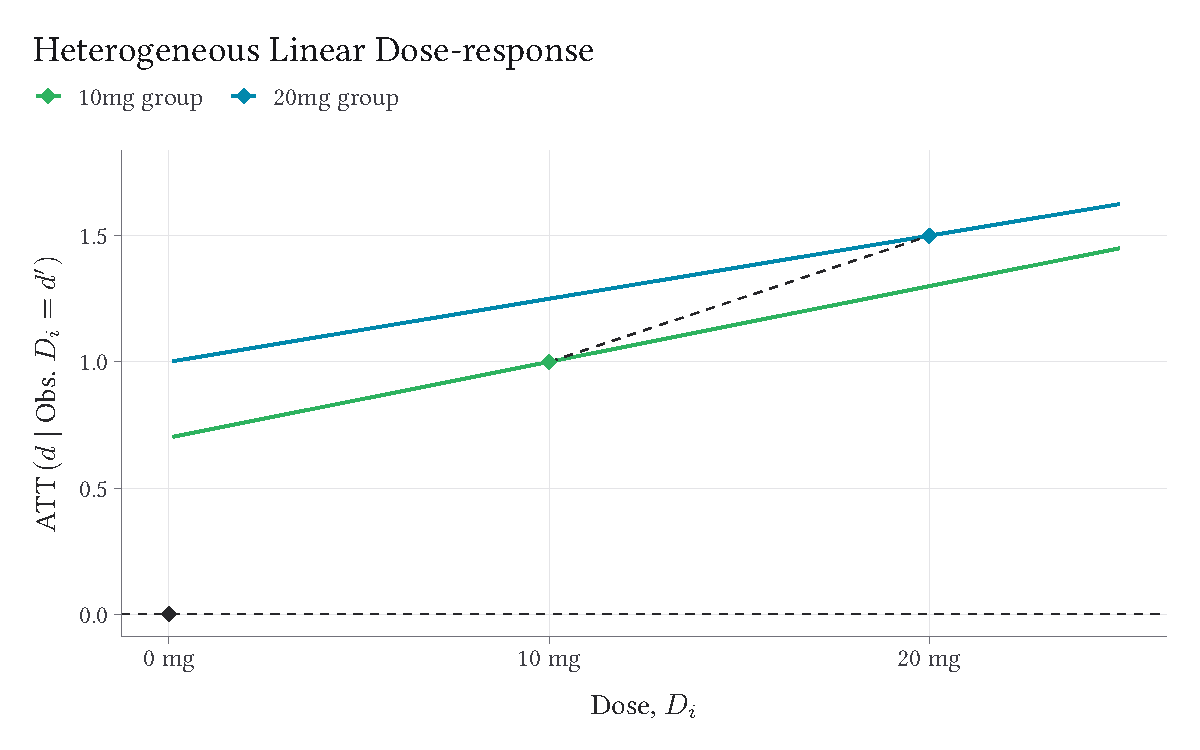
\includegraphics[width=0.78\textwidth,height=0.70\textheight,keepaspectratio]{figures/dxt/discrete_te_linear_het.pdf}
\end{center}
\begin{center}
\footnotesize\color{warmgray}\itshape
Same average response, but the dose-1 group reacts more than dose-2's first-pill response would have predicted. \;Heterogeneity in returns to dose.
\end{center}
\end{frame}

\begin{frame}{Discrete: first differences make the comparison visible}
\begin{center}
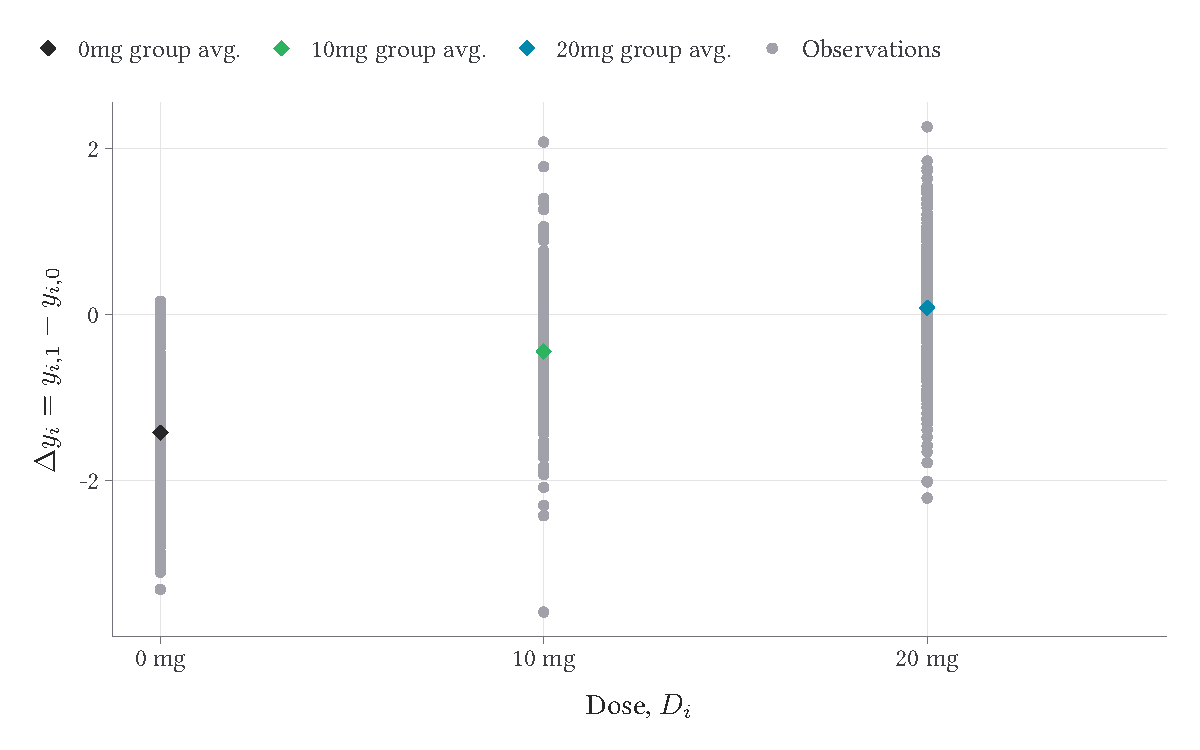
\includegraphics[width=0.78\textwidth,height=0.70\textheight,keepaspectratio]{figures/dxt/discrete_raw_first_differences.pdf}
\end{center}
\begin{center}
\footnotesize\color{warmgray}\itshape
$\Delta Y$ for each dose group. \;A clean way to read the pre-period (should be flat) vs the post-period (the treatment effect).
\end{center}
\end{frame}

\begin{frame}{Discrete: the implied counterfactual}
\begin{center}
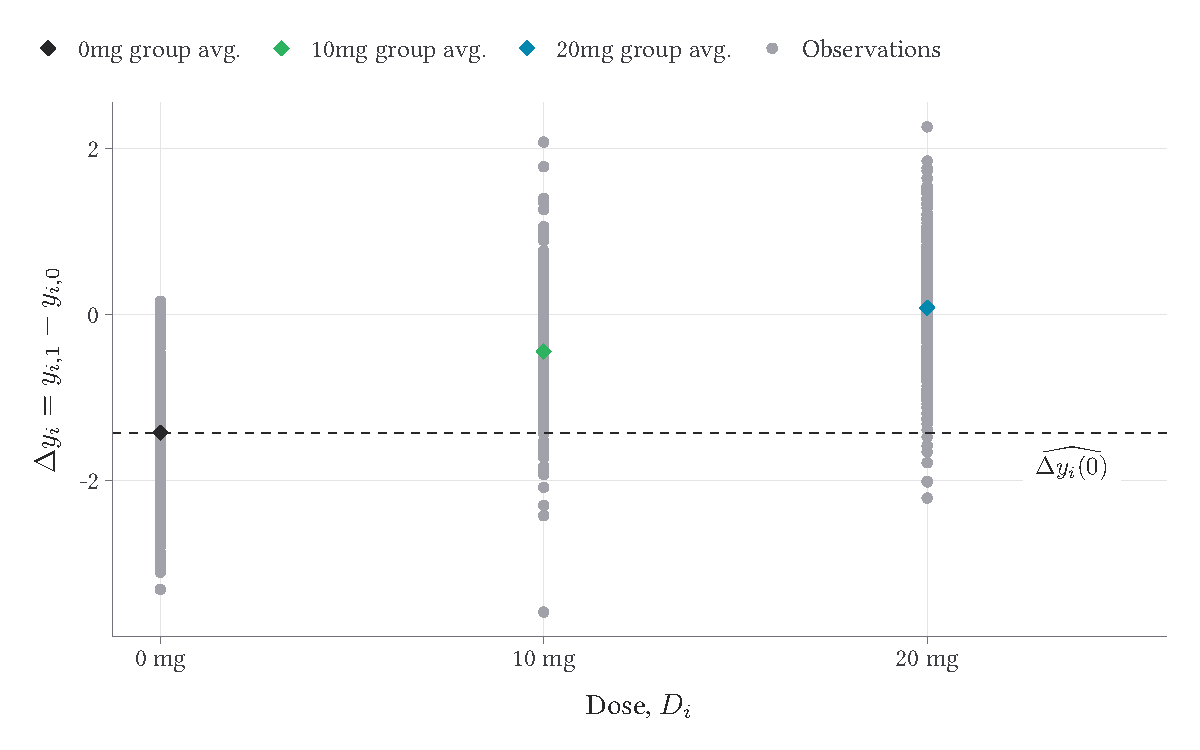
\includegraphics[width=0.78\textwidth,height=0.70\textheight,keepaspectratio]{figures/dxt/discrete_implied_counterfactual.pdf}
\end{center}
\begin{center}
\footnotesize\color{warmgray}\itshape
The dashed lines show what dose-1 and dose-2 \textit{would have looked like} absent treatment --- constructed under standard PT.
\end{center}
\end{frame}

\begin{frame}{Discrete: the DiD estimates, dose by dose}
\begin{center}
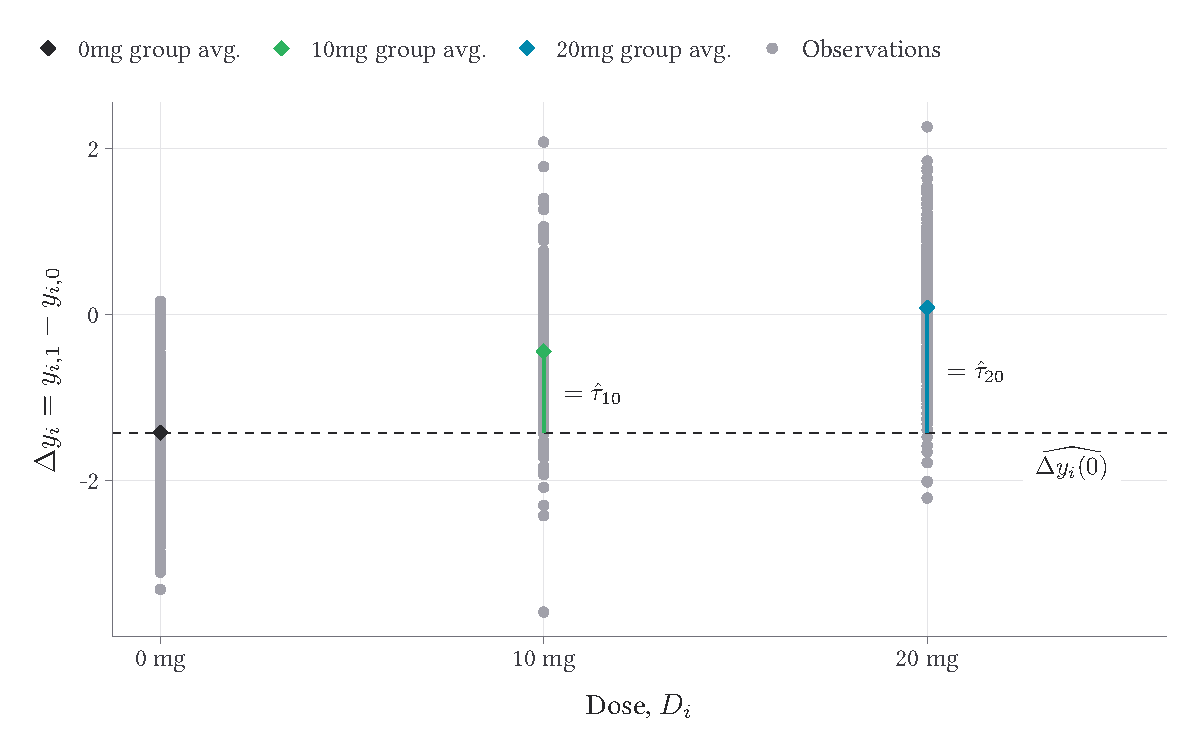
\includegraphics[width=0.78\textwidth,height=0.70\textheight,keepaspectratio]{figures/dxt/discrete_did_estimates.pdf}
\end{center}
\begin{center}
\footnotesize\color{warmgray}\itshape
Each treated dose-group's DiD versus the never-treated: $\widehat{\text{ATT}}(1 \mid 1)$ and $\widehat{\text{ATT}}(2 \mid 2)$. \;Two separate point estimates, one per dose.
\end{center}
\end{frame}

\begin{frame}{Recap of Part 2}
\vspace{0.2cm}

\begin{itemize}\setlength\itemsep{4pt}
  \item Two target parameters: \;\textbf{ATT($d \mid d$)} (level) and \;\textbf{ACRT($d$)} (slope).
  \item Standard PT identifies the level curve.
  \item Strong PT --- ruling out selection on dose response --- identifies the ACRT.
  \item Discrete multi-valued case gives finite-group intuition; continuous extends the same logic to a curve.
\end{itemize}

\vspace{0.5cm}

\highlight{Part 3 estimates these objects, with three options: overall ATT, bins, and non-parametric smoothing.}
\end{frame}

% =============================================================================
% PART IV — Estimation
% =============================================================================

\remixsection{Part 3: \\ Estimation}

%% ---------- Backwards vs. Forwards engineering ----------
\begin{frame}{Backwards engineering vs.\ Forwards engineering}
\vspace{0em}

\begin{columns}[T]

\begin{column}{0.46\textwidth}
\textbf{\color{red!70!black}Backwards}
\vspace{0.1em}
\begin{itemize}\setlength\itemsep{0pt}\footnotesize
  \item Run TWFE; let OLS hand you a number.
  \item FWL: that number is a weighted average of dose effects.
  \item Weights come from $\text{Var}(D \mid \text{controls})$.
  \item Some weights are \textbf{negative}; they shift across the dose distribution.
  \item No causal parameter in sight.
\end{itemize}
\end{column}

\begin{column}{0.06\textwidth}
\begin{center}
\vspace{2em}
\color{warmgray}\Large$\to$
\end{center}
\end{column}

\begin{column}{0.47\textwidth}
\textbf{\color{remixgreendark}Forwards}
\vspace{0.1em}
\begin{itemize}\setlength\itemsep{0pt}\footnotesize
  \item Name the target: $\text{ATT}(d \mid d)$ or $\text{ACRT}(d)$.
  \item State assumptions you'll defend.
  \item Build an estimator that's right on average under those assumptions.
  \item Meaning of the estimate is known \textit{before} you run it.
\end{itemize}
\end{column}

\end{columns}

\vspace{0.5em}
\begin{center}
\highlight{CBS is forwards. \;TWFE with continuous $D$ is backwards.}
\end{center}
\end{frame}

%% ---------- A familiar precedent: Wald IV and the LATE ----------
\begin{frame}{A familiar precedent: Wald IV and the LATE}
\vspace{0.1em}

The ATE had long been the target parameter.

\vspace{0.4em}

\begin{itemize}\setlength\itemsep{3pt}\footnotesize
  \item Imbens \& Angrist (1994) started with an estimator --- Wald IV --- and worked out what it actually identifies under heterogeneous effects: the \textbf{LATE}, the average effect among compliers.
  \item They met opposition. The LATE wasn't the ATE; critics argued you couldn't pick it ex ante.
  \item Eventually the field came around. Today: name the target (LATE, ATT, $\ldots$) \textit{first}, then build the estimator.
  \item We're doing the same move here. TWFE on continuous $D$ isn't the ATT. \;Pick $\text{ATT}(d \mid d)$ or $\text{ACRT}(d)$; then estimate.
\end{itemize}

\vspace{0.3em}
\begin{center}
{\footnotesize\color{warmgray}
\href{https://www.youtube.com/watch?v=QnwTdd-7BvY}%
{\texttt{youtube.com/watch?v=QnwTdd-7BvY}}}
\end{center}
\end{frame}

\begin{frame}{Three estimation options for ATT($d \mid d$)}
\vspace{0.2cm}

Given continuous $D$, three practical strategies:

\vspace{0.4cm}

\begin{enumerate}\setlength\itemsep{5pt}
  \item \textbf{Overall ATT.} \;Average $\text{ATT}(d \mid d)$ across the treated. \;One number.
  \item \textbf{Bins.} \;Partition the dose into intervals; estimate one ATT per bin. \;A coarse dose-response curve.
  \item \textbf{Non-parametric smoothing.} \;A continuous dose-response function $\widehat{\text{ATT}}(\cdot)$ via kernels or splines.
\end{enumerate}

\vspace{0.4em}
\meta{Each one is a different point on the bias-variance-interpretability trade-off.}
\end{frame}

\begin{frame}{Option 1: Overall ATT --- one number summary}
\vspace{0.2cm}

\textbf{Definition.}
\[
\overline{\text{ATT}} \;=\; \mathbb{E}\big[\,\text{ATT}(D_i \mid D_i) \mid D_i > 0\,\big]
\]

\vspace{0.4cm}

The average of the dose-specific ATTs, taken over the treated dose distribution. \;The weight is the density $f_D$ --- not the level weight or any other formula.

\vspace{0.4cm}

\textbf{When to use it.} \;When the audience wants a single headline ATT. \;When the dose response is not the object of interest. \;When precision matters more than dose-by-dose detail.

\vspace{0.3em}
\meta{This is what most empirical papers want, but it is \textit{not} what TWFE delivers.}
\end{frame}

\begin{frame}{Option 2: Bins --- a coarse dose-response curve}
\vspace{0.1cm}
\begin{center}
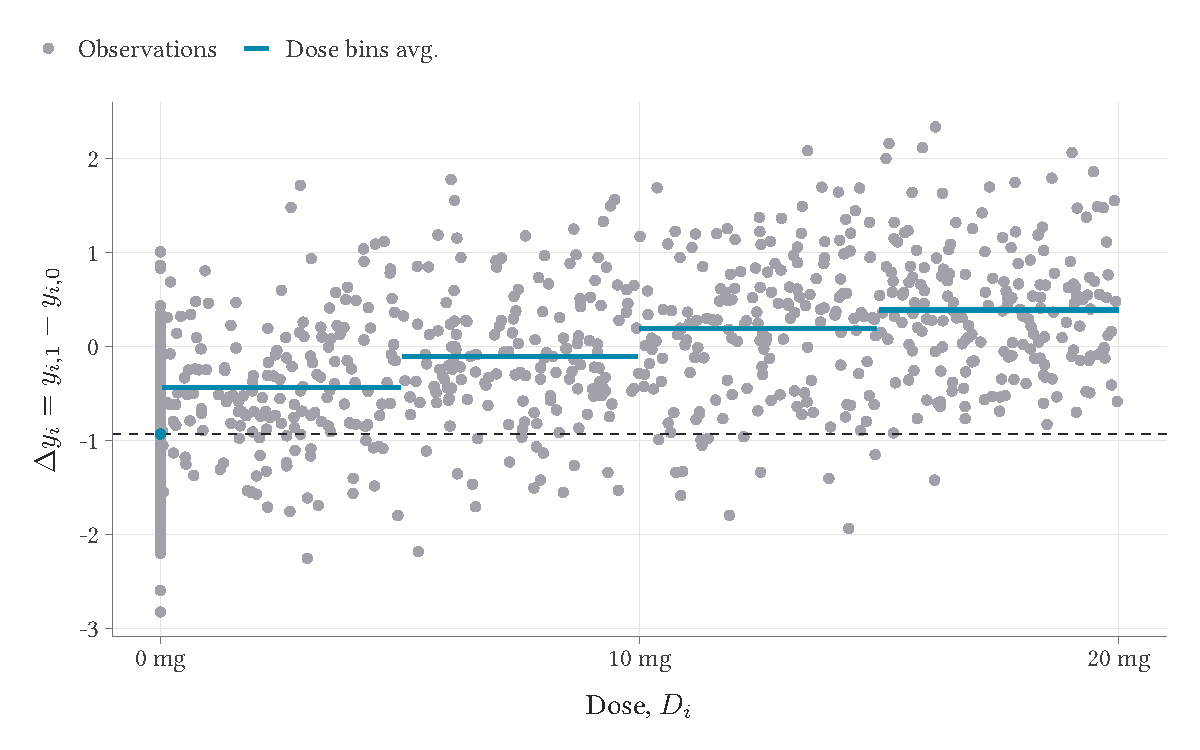
\includegraphics[width=0.78\textwidth,height=0.66\textheight,keepaspectratio]{figures/dxt/continuous_binned_avgs.pdf}
\end{center}
\vspace{0.2em}
\begin{center}
\scriptsize\color{warmgray}\itshape
Partition dose into intervals. \;Estimate one ATT per bin. \;Step-function dose response.
\end{center}
\end{frame}

\begin{frame}{Pros and cons of bins}
\vspace{0.1cm}

\textbf{Pros.}
\begin{itemize}\footnotesize\setlength\itemsep{0pt}
  \item Easy to estimate; nothing more than a series of 2$\times$2's.
  \item Easy to communicate: ``effect at 5--10\% cut was X.''
  \item Bins can be chosen with policy thresholds in mind.
  \item Identified under \textit{standard} parallel trends --- no need for Strong PT.
\end{itemize}

\vspace{0.3cm}

\textbf{Cons.}
\begin{itemize}\footnotesize\setlength\itemsep{0pt}
  \item Inside a bin you average over a range of doses --- losing within-bin variation.
  \item Choice of bin width is a discretion knob.
  \item No standard error on the dose-response curve as a continuous object.
\end{itemize}

\vspace{0.3em}
\highlight{Often the right first cut. \;Rarely the final analysis.}
\end{frame}

%% ---------- Why not shrink the bins? ----------
\begin{frame}{Why not just shrink the bins?}
\vspace{0.6em}

If bins of width $h$ work, why not let $h \to 0$ and recover a curve?

\vspace{1em}

\begin{itemize}\setlength\itemsep{0.5em}
  \item Each bin holds fewer observations as $h$ shrinks. \;The bin average gets noisier.
  \item Variance grows faster than bias falls. \;The estimator stops converging.
  \item Inside a bin the slope is zero. \;You can't read $\text{ACRT}(d)$ off a step function.
  \item Step functions don't have derivatives. \;You can't take limits.
\end{itemize}

\vspace{0.6em}
\begin{center}
\highlight{Fine bins are not the answer. \;We need a smooth curve.}
\end{center}
\end{frame}

%% ---------- Splines ----------

%% Slide 1: visual — what are pieces?
\begin{frame}{Splines: the curve is made of pieces}
\vspace{0.1cm}
\begin{center}
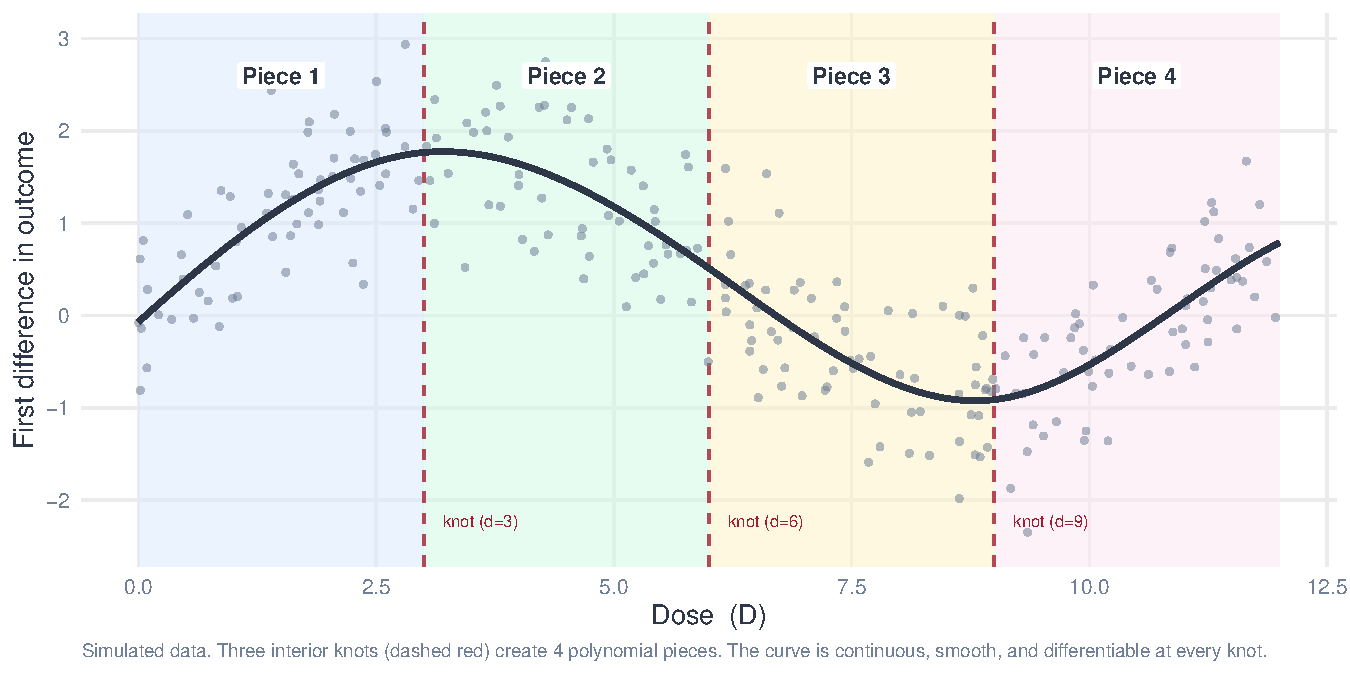
\includegraphics[width=0.84\textwidth,height=0.68\textheight,keepaspectratio]{figures/dxt/spline_pieces.pdf}
\end{center}
\vspace{-0.2cm}
\begin{center}
\footnotesize\color{warmgray}\itshape
3 knots divide the dose range into 4 regions. Inside each region: one cubic polynomial. \\
The curve is forced to match in value, slope, and curvature at every knot.
\end{center}
\end{frame}

%% Slide 2: Stata code
\begin{frame}[fragile]{Fitting a spline in Stata: \texttt{mkspline}}

\texttt{mkspline} generates the basis columns; \texttt{reg} does the rest.

\vspace{0.3em}

\begin{lstlisting}[language=Stata,basicstyle=\ttfamily\footnotesize]
* 1. Make the basis  (4 quantile knots = 3 interior knots = 4 pieces)
mkspline spl = dose, nknots(4) cubic displayknots

* 2. Regress the first-differenced outcome on the basis
reg delta_y spl*

* 3. Fitted values and plot
predict yhat, xb
twoway (scatter delta_y dose, mcolor(gs10) msize(small)) ///
       (line yhat dose, sort lcolor(navy) lwidth(medthick)), ///
       xtitle("Dose") ytitle("First difference") legend(off)
\end{lstlisting}

\vspace{0.15em}
\meta{\texttt{nknots(4)} places knots at dose quantiles. \;\texttt{displayknots} prints their values so you can report them.}
\end{frame}

%% Slide 3: what the fitted values look like
\begin{frame}{What the spline estimates}
\vspace{0.1cm}
\begin{center}
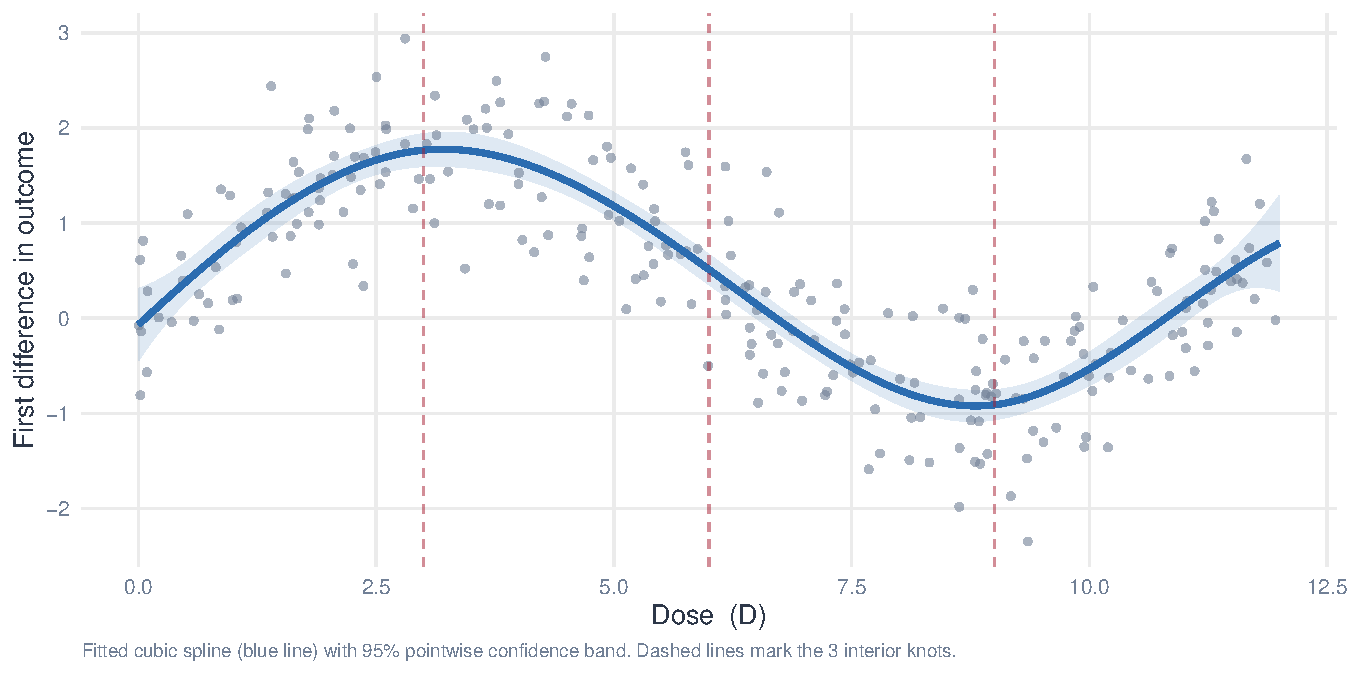
\includegraphics[width=0.84\textwidth,height=0.68\textheight,keepaspectratio]{figures/dxt/spline_fitted.pdf}
\end{center}
\vspace{-0.2cm}
\begin{center}
\footnotesize\color{warmgray}\itshape
The \texttt{predict yhat} line from the regression above. One smooth curve through the scatter. \\
Pointwise confidence band from \texttt{predict se, stdp} and \texttt{twoway rarea}.
\end{center}
\end{frame}

%% ---------- Kernel regression ----------
\begin{frame}{Kernel regression: another way to smooth}
\vspace{0.6em}

At each dose $d$, average outcomes from nearby observations, weighted by a kernel:
\[
\widehat m(d) \;=\; \frac{\sum_i K_h(D_i - d) \cdot \Delta\tilde Y_i}{\sum_i K_h(D_i - d)}
\]

\vspace{0.6em}

\begin{itemize}\setlength\itemsep{0.3em}
  \item $K$ is a weight function (Gaussian, Epanechnikov, $\ldots$).
  \item Bandwidth $h$ controls smoothness. \;Small $h$ = local, noisy. \;Large $h$ = smooth, biased.
\end{itemize}

\vspace{0.7em}
\begin{center}
\highlight{Splines fit globally with $K$ knots. \;Kernels fit locally with a bandwidth. \;Same goal.}
\end{center}
\end{frame}

%% ---------- Kernel: bandwidth picture ----------
\begin{frame}{Bandwidth controls smoothness}
\vspace{0.1cm}
\begin{center}
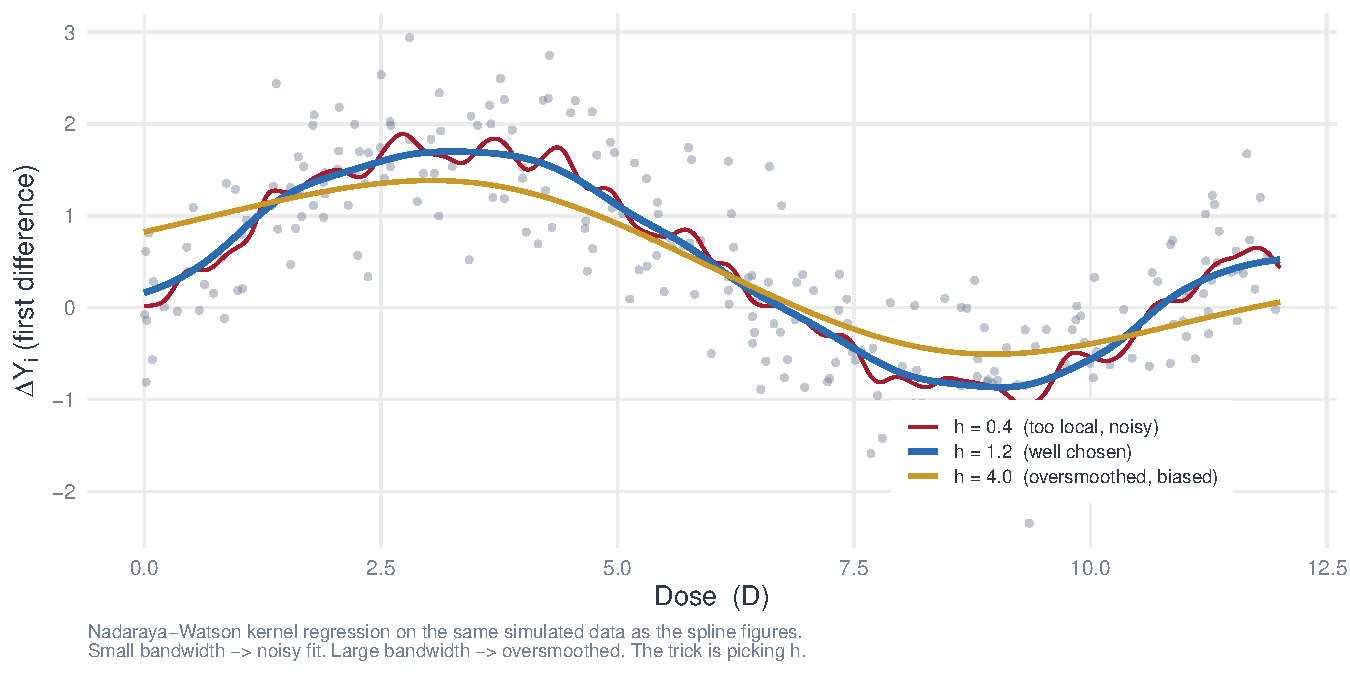
\includegraphics[width=0.92\textwidth,height=0.66\textheight,keepaspectratio]{figures/dxt/kernel_bandwidth.pdf}
\end{center}
\vspace{0.2em}
\begin{center}
\scriptsize\color{warmgray}\itshape
Same simulated data as the spline figure. \;Three bandwidths. \;The trick is picking $h$.
\end{center}
\end{frame}

%% ---------- Fitting kernel regression in Stata ----------
\begin{frame}[fragile]{Fitting kernel regression in Stata: \texttt{lpoly}}

\texttt{lpoly} fits a local polynomial; \texttt{degree(0)} gives Nadaraya--Watson.

\vspace{0.3em}

\begin{lstlisting}[language=Stata,basicstyle=\ttfamily\footnotesize]
* Local-linear (degree 1) kernel fit on a grid of doses
lpoly delta_y dose, kernel(epanechnikov) degree(1) ///
      bwidth(1.2) generate(dgrid yhat) se(se_yhat)

* Plot the fit with a 95% pointwise band
gen lo = yhat - 1.96*se_yhat
gen hi = yhat + 1.96*se_yhat
twoway (rarea lo hi dgrid, color(green%20)) ///
       (scatter delta_y dose, mcolor(gs10) msize(small)) ///
       (line yhat dgrid, sort lcolor(dkgreen) lwidth(medthick)), ///
       xtitle("Dose") ytitle("First difference") legend(off)
\end{lstlisting}

\vspace{0.15em}
\meta{\texttt{bwidth(.)} picks the bandwidth by rule-of-thumb. \;Use cross-validation for a data-driven choice.}
\end{frame}

%% ---------- What the kernel estimates ----------
\begin{frame}{What the kernel regression estimates}
\vspace{0.1cm}
\begin{center}
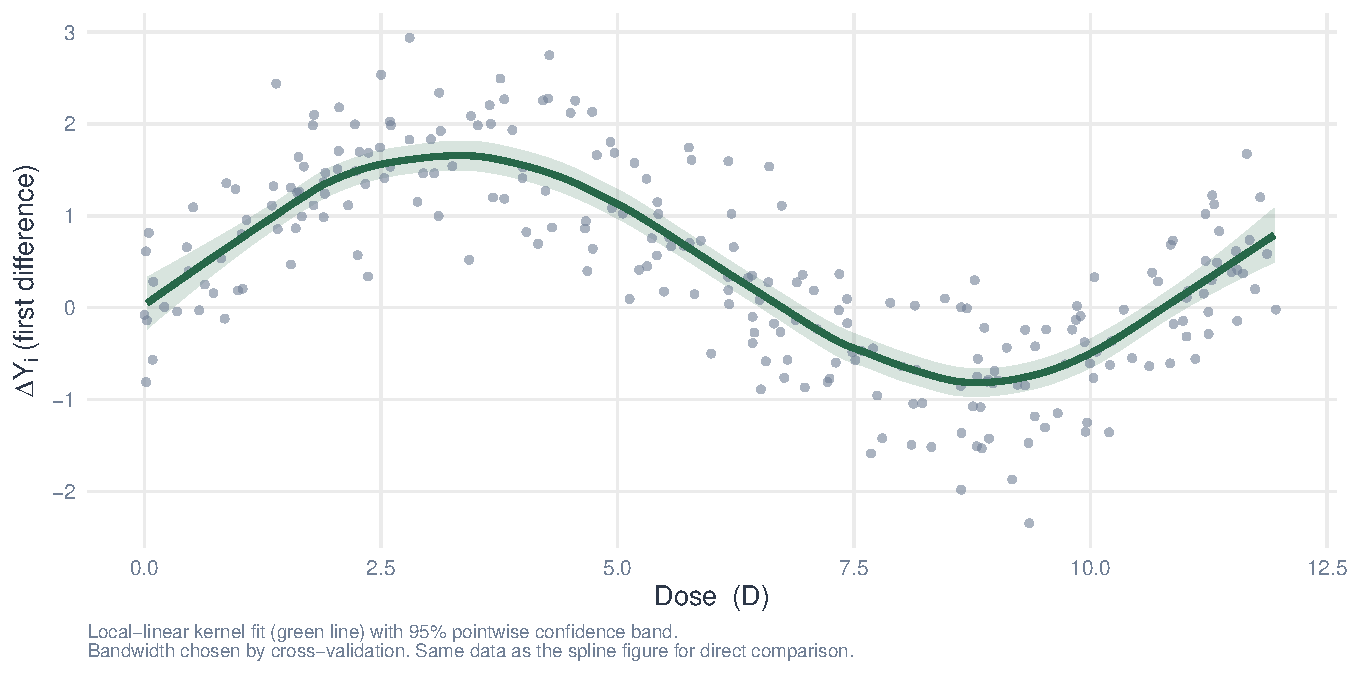
\includegraphics[width=0.92\textwidth,height=0.66\textheight,keepaspectratio]{figures/dxt/kernel_fitted.pdf}
\end{center}
\vspace{0.2em}
\begin{center}
\scriptsize\color{warmgray}\itshape
Local-linear kernel fit with 95\% pointwise band. \;Compare to the spline fit on the same data --- the curves are nearly indistinguishable.
\end{center}
\end{frame}

%% ---------- A detour: where the spline machinery comes from ----------
\begin{frame}{Where does the spline machinery come from?}
\vspace{0.3em}

Estimating $\text{ATT}(d \mid d)$ as a smooth function of $d$ is a classical nonparametric problem. \;The tools are not new.

\vspace{0.6em}

\textbf{Sieve regression} (Grenander 1981; Chen 2007 \textit{Handbook}). \;Approximate an unknown function by a finite-dimensional basis --- B-splines, polynomials, wavelets --- and let the basis grow with the sample. \;Bias falls as you add terms; variance is controlled by how fast.

\vspace{0.6em}

\textbf{Uniform inference} (Chen \& Christensen 2018 \textit{QE}; Chen, Christensen \& Kankanala 2024). \;Honest \textit{confidence bands} that cover the whole curve at once --- so you can say ``the dose-response is positive on $[d_1, d_2]$.''

\vspace{0.5em}
\begin{center}
\highlight{What's new in CBS isn't the estimator. \;It's the identification.}
\end{center}
\end{frame}

%% ---------- CBS methodology ----------
\begin{frame}{CBS use B-spline sieve regression}
\vspace{0.6em}

The \texttt{contdid} package implements CBS's recipe. \;It wraps Chen--Christensen--Kankanala's \texttt{npiv}.

\vspace{0.6em}

Three steps:
\begin{enumerate}\setlength\itemsep{0.25em}\footnotesize
  \item Center the outcome: \;$\Delta\tilde Y_i = \Delta Y_i - \widehat m(0)$, \;where $\widehat m(0)$ is the average $\Delta Y$ for untreated units.
  \item Regress $\Delta\tilde Y_i$ on the B-spline basis $\psi(D_i)$, \;using only treated units ($D_i > 0$).
  \begin{itemize}\setlength\itemsep{0.1em}
    \item The ``B'' is for \textbf{basis}: \;$\psi(d) = (\psi_1(d), \ldots, \psi_K(d))$ is $K$ basis functions built from the knots.
    \item Knots set the structure; the basis is the columns you regress on (\texttt{mkspline} in Stata).
  \end{itemize}
  \item Bootstrap for pointwise confidence bands on the fitted $\widehat{\text{ATT}}(d \mid d)$ curve.
\end{enumerate}
\end{frame}

%% ---------- Assumptions ----------
\begin{frame}{What we have to assume}
\vspace{0.4em}

\begin{itemize}\setlength\itemsep{0.7em}
  \item \textbf{Strong parallel trends.} \;$E[\Delta Y(0) \mid D = d] = E[\Delta Y(0) \mid D = 0]$ for \textit{every} $d$ --- not just $d = 0$ vs.\ $d > 0$. \;Rules out selection-on-dose-response.
  \item \textbf{Smoothness of $\text{ATT}(d \mid d)$.} \;Continuous, bounded derivative in $d$. \;The sieve approximates a smooth function, not arbitrary jumps.
  \item \textbf{Overlap.} \;Enough observations near every $d$ where the curve is estimated.
  \item \textbf{Tuning chosen sensibly.} \;Number of knots from cross-validation or a rule of thumb.
\end{itemize}

\vspace{0.4em}
\begin{center}
\highlight{Strong PT is the load-bearing assumption. \;The rest are technical.}
\end{center}
\end{frame}

%% ---------- The formula ----------
\begin{frame}{The estimator, formally}
\vspace{0.7em}

Let $\psi(d) = (\psi_1(d), \ldots, \psi_K(d))^\top$ be the cubic B-spline basis at dose $d$.

\vspace{0.9em}

Fit OLS on the treated units:
\[
\widehat\theta \;=\; \arg\min_\theta \;\sum_{i: D_i > 0} \big(\Delta\tilde Y_i - \theta^\top \psi(D_i)\big)^2
\]

\vspace{0.9em}

The dose-response curve and its derivative:
\[
\widehat{\text{ATT}}(d \mid d) \;=\; \widehat\theta^\top \psi(d)
\qquad
\widehat{\text{ACRT}}(d) \;=\; \widehat\theta^\top \psi'(d)
\]

\vspace{0.5em}
\begin{center}
\highlight{One regression delivers both target parameters.}
\end{center}
\end{frame}

%% ---------- Option 3: Non-parametric smoothing (figure) ----------
\begin{frame}{Option 3: Non-parametric smoothing}
\vspace{0.1cm}
\begin{center}
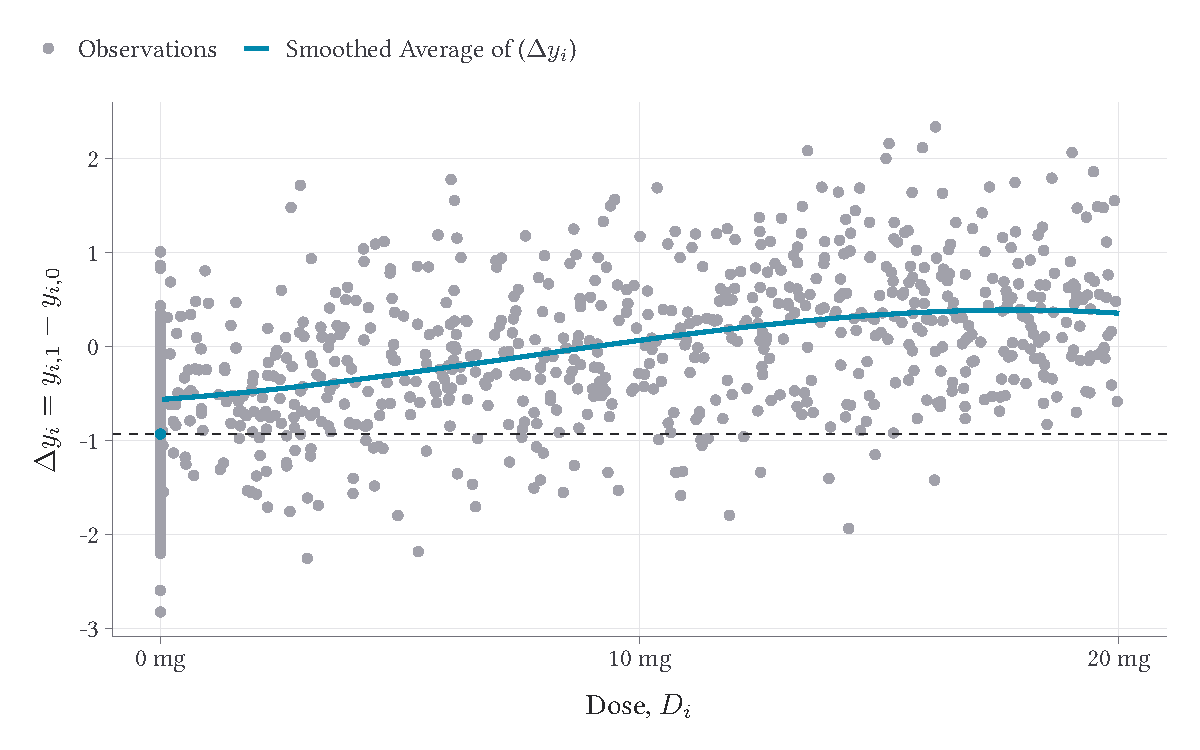
\includegraphics[width=0.74\textwidth,height=0.62\textheight,keepaspectratio]{figures/dxt/continuous_smoothed_avgs.pdf}
\end{center}
\vspace{0.3em}
\begin{center}
\footnotesize\color{warmgray}\itshape
A continuous $\widehat{\text{ATT}}(\cdot)$ over the dose range, with pointwise confidence bands.
\end{center}
\end{frame}

\begin{frame}[fragile]{The \texttt{contdid} package}
\vspace{0.2cm}

Brantly Callaway's R package \texttt{contdid} implements all three options.

\begin{lstlisting}[language=Rcode]
library(contdid)
result <- cont_did(
  yname = "outcome", tname = "year", idname = "unit_id",
  dname = "dose",    gname = "treatment_timing",
  data = panel_data,
  target_parameter  = "level",     # "level" = ATT(d|d); "derivative" = ACRT
  aggregation       = "dose",      # or "overall"
  control_group     = "notyettreated"
)
summary(result)
ggcont_did(result, type = "att")
\end{lstlisting}

\vspace{0.1em}
\meta{\texttt{"derivative"} requires strong PT; \texttt{"level"} only standard PT.}
\end{frame}

\begin{frame}{Pros and cons of non-parametric smoothing}
\vspace{0.2cm}

\textbf{Pros.}
\begin{itemize}\small\setlength\itemsep{1pt}
  \item Returns a continuous function, not a step.
  \item Confidence bands.
  \item Less ad-hoc than bin choice.
\end{itemize}

\vspace{0.4cm}

\textbf{Cons.}
\begin{itemize}\small\setlength\itemsep{1pt}
  \item Bandwidth/smoothing choice is the new discretion.
  \item Curse of dimensionality at the tails of the dose distribution.
  \item Harder to communicate to a non-technical audience.
\end{itemize}

\vspace{0.3em}
\meta{In practice: bin first, smooth second, report both.}
\end{frame}

\begin{frame}{The WTO example, done properly}
\vspace{0.1cm}
\begin{center}
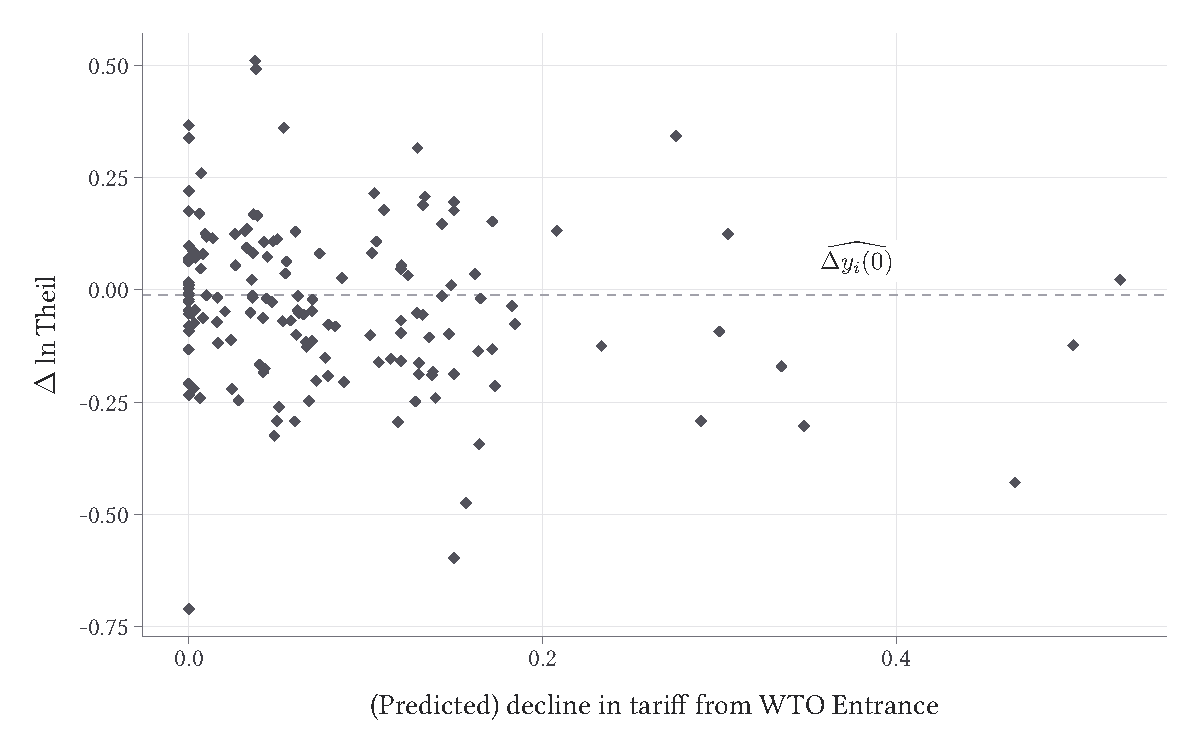
\includegraphics[width=0.78\textwidth,height=0.70\textheight,keepaspectratio]{figures/dxt/china_wto_raw.pdf}
\end{center}
\vspace{-0.05cm}
\begin{center}
\footnotesize\color{warmgray}\itshape
Raw outcome trajectories by tariff-cut group; the setup before any DiD.
\end{center}
\end{frame}

\begin{frame}{The dose-response estimates}
\vspace{0.1cm}
\begin{center}
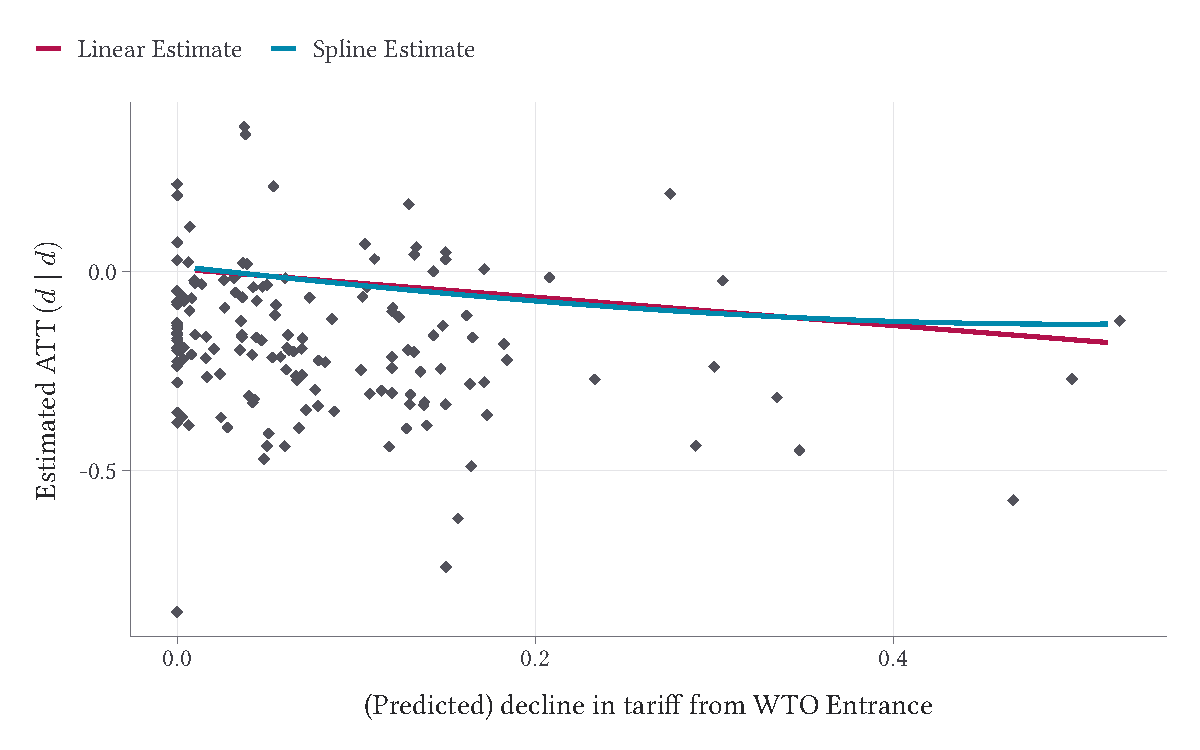
\includegraphics[width=0.78\textwidth,height=0.70\textheight,keepaspectratio]{figures/dxt/china_wto_ests.pdf}
\end{center}
\vspace{-0.05cm}
\begin{center}
\footnotesize\color{warmgray}\itshape
$\widehat{\text{ATT}}(d \mid d)$ across the dose distribution. \;A real curve, not the single $-0.322$ that TWFE delivers.
\end{center}
\end{frame}

\begin{frame}{Pre-trends, dose by dose}
\vspace{0.1cm}
\begin{center}
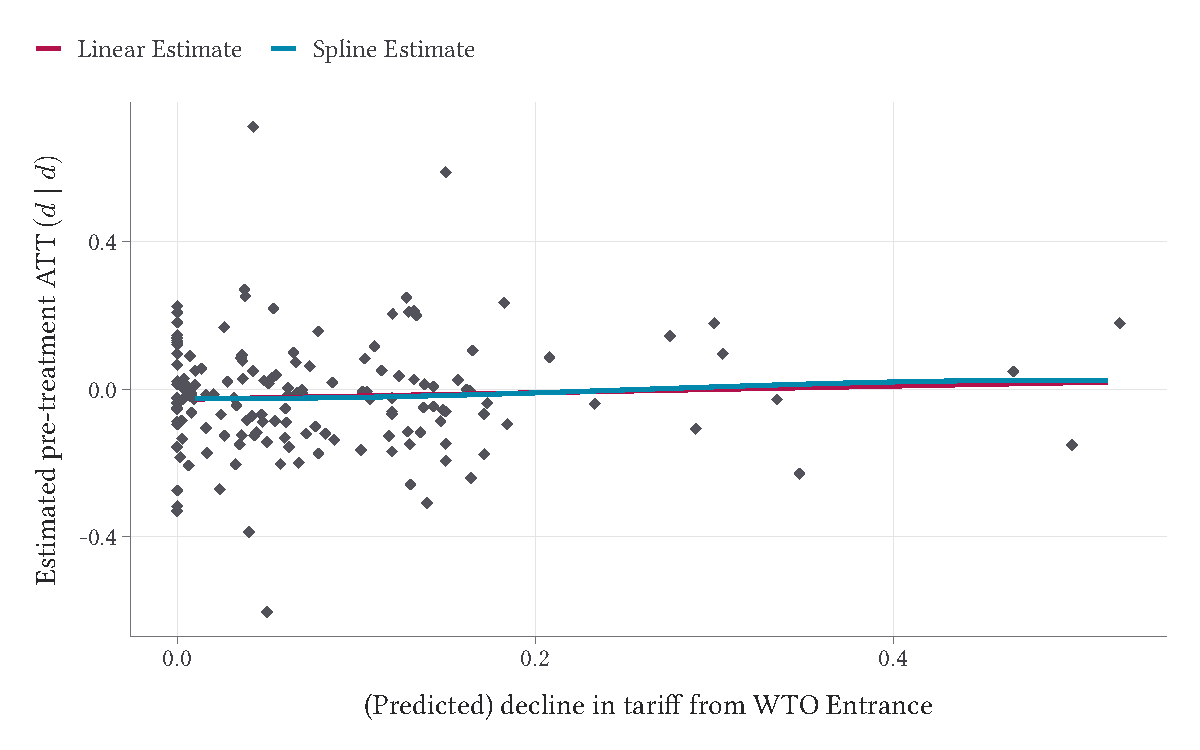
\includegraphics[width=0.78\textwidth,height=0.70\textheight,keepaspectratio]{figures/dxt/china_wto_pretrends_ests.pdf}
\end{center}
\vspace{-0.05cm}
\begin{center}
\footnotesize\color{warmgray}\itshape
Pre-period placebos: should be near zero under standard PT.
\end{center}
\end{frame}

\begin{frame}{Closing: what to do tomorrow}
\vspace{0.2cm}

\textbf{Don't run TWFE with a continuous dose and report $\widehat\beta$ as ``the dose effect.''} \;Under heterogeneity, $\widehat\beta^{\text{twfe}}$ is a weighted average with sign-flipping weights, scaled by features of the dose distribution that have nothing to do with the causal question.

\vspace{0.4cm}

\textbf{Do:}
\begin{itemize}\small\setlength\itemsep{1pt}
  \item Pick a target parameter: \;\textbf{ATT($d \mid d$)} or \textbf{ACRT($d$)}.
  \item Estimate that parameter: overall, bins, or non-parametric.
  \item State the identifying assumption: standard PT or strong PT.
  \item Report pre-trend placebos at each dose.
\end{itemize}

\vspace{0.4em}
\highlight{The continuous DiD machinery is now available --- and the cost of doing it right is no longer prohibitive.}
\end{frame}

\end{document}
